%You can delete all the comments after you have finished your document
%this sets up the defaults for the documents, 12pt font and A4 size. The article type sets this up as such as opposed to letter or memo.

%for the finer points LaTeX see https://en.wikibooks.org/wiki/LaTeX or http://tex.stackexchange.com/

\documentclass[12pt,a4paper]{article}
\usepackage{titlesec} %these are how we import packages, one helps set up footers and title layout
\usepackage{fancyhdr}

% !TEX TS-program = pdflatex
% !TEX encoding = UTF-8 Unicode
\usepackage[utf8]{inputenc} % set input encoding (not needed with XeLaTeX)

\usepackage{graphicx} % support the \includegraphics command and options
\graphicspath{{./images/}}

\usepackage[parfill]{parskip} % Activate to begin paragraphs with an empty line rather than an indent

%%% PACKAGES
\usepackage{booktabs} % for much better looking tables
\usepackage{array} % for better arrays (eg matrices) in maths
\usepackage{paralist} % very flexible & customisable lists (eg. enumerate/itemize, etc.)
\usepackage{verbatim} % adds environment for commenting out blocks of text & for better verbatim
\usepackage{subfig} % make it possible to include more than one captioned figure/table in a single float
\usepackage[toc,page]{appendix}
\usepackage{xcolor}
\usepackage[hidelinks,breaklinks,colorlinks,linkcolor={black},citecolor={blue!80!black},urlcolor={blue!80!black}]{hyperref} % make citations clickable links
\usepackage{apalike} 

\newcommand{\myparagraph}[1]{\paragraph{#1}\mbox{}\\} %put paragraph headings on their own line!

%header and footer settings
\pagestyle{fancyplain}
\fancyhf{}
\renewcommand{\headrulewidth}{0.5pt}
\renewcommand{\footrulewidth}{0.5pt}
\setlength{\headheight}{15pt}
\fancyhead[L]{Svetlozar Georgiev - 40203970}
\fancyhead[R]{SOC10101 Honours Project}
\fancyfoot[L]{}
\fancyfoot[C]{\thepage}

%set better section layout
\makeatletter
\renewcommand\subsection{\@startsection {subsection}{1}{2mm} % name, level, indent
                               {3pt plus 2pt minus 1pt} % before skip
                               {3pt plus 0pt} % after skip
                               {\normalfont\bfseries}}
\makeatother
\makeatletter
\renewcommand\section{\@startsection {section}{1}{0mm} % name, level, indent
                               {4pt plus 2pt minus 1pt} % before skip
                               {4pt plus 0pt} % after skip
                               {\bfseries}}
\makeatother

 % macro for adding figures more easily
\newcommand{\figuremacro}[5]{
    \begin{figure}[#1]
        \centering
        \caption[#3]{\textbf{#3}#4}
        \includegraphics[width=#5\columnwidth]{#2}
        \label{fig:#2}
    \end{figure}
}

%this starts the document
\begin{document}

%you can import other documents into your main one, these layout the Title and Declarations on its own page.
%you might need to change these to \ if your on Microsoft Windows.
\newcommand{\HRule}{\rule{\linewidth}{0.5mm}}

\begin{titlepage}
	\begin{center}

	\HRule \\[0.4cm]
    	{\Large \bfseries The Title of Your Dissertation\par}
	\vspace{0.2cm}
	\HRule \\[1.5cm]

	
    	\vspace{3cm}
	\begin{minipage}{0.4\textwidth}
	\begin{center} \large
        \emph{}\\
        	Svetlozar Georgiev - 40203970
				
   	 \end{center}
    	\end{minipage}
	
	\vspace{2cm}
    	\begin{minipage}{1\textwidth}
    	\begin{center} \large
        
		Submitted in partial fulfilment of \\
		the requirements of Edinburgh Napier University \\
		for the Degree of \\
        	BEng (Hons) Software Engineering
    	\end{center}
    	\end{minipage}

    	\vfill

    	% Bottom of the page
	\begin{minipage}{1\textwidth}
    	\begin{center} \large
		School of Computing
    	\end{center}
    	\end{minipage}
	
	\vspace{1cm}
    	{\large \today}


	\end{center}
\end{titlepage}
%{\large Submitted in partial fulfilment of the requirements of Edinburgh Napier University for the Degree of }

\section*{Authorship Declaration}
\vspace{0.5cm}
\begin{flushleft}
I, Svetlozar Georgiev Georgiev, confirm that this dissertation and the work presented in it are my own achievement.\newline

Where I have consulted the published work of others this is always clearly attributed;\newline

Where I have quoted from the work of others the source is always given. With the exception of such quotations this dissertation is entirely my own work;\newline

I have acknowledged all main sources of help; \newline

If my research follows on from previous work or is part of a larger collaborative research project I have made clear exactly what was done by others and what I have contributed myself;\newline

I have read and understand the penalties associated with Academic Misconduct.\newline

I also confirm that I have obtained informed consent from all people I have involved in the work in this dissertation following the School's ethical guidelines.\newline
\end{flushleft}

\begin{flushleft} \large
\emph{Signed:} \\
\end{flushleft}

\vspace{.5cm}

\begin{flushleft} \large
\emph{Date:} \\
\end{flushleft}

\vspace{.5cm}

\begin{flushleft} \large
\emph{Matriculation no: 40203970}  \\
\end{flushleft}
\pagebreak

\section*{General Data Protection Regulation Declaration}
\vspace{0.5cm}
\begin{flushleft}
Under the General Data Protection Regulation (GDPR) (EU) 2016/679, the University cannot disclose your grade to an unauthorised person. However, other students benefit from studying dissertations that have their grades attached. \newline

\vspace{0.5cm}

Please sign your name below one of the options below to state your preference.\newline
\vspace{0.5cm}

The University may make this dissertation, with indicative grade, available to others.\newline
\vspace{3cm}


The University may make this dissertation available to others, but the grade may not be disclosed.\newline
\vspace{3cm}


The University may not make this dissertation available to others.\newline
\end{flushleft}



\pagebreak

%LaTeX let you define the abstract separately so it wont get sucked into the main document.
\begin{abstract}
\end{abstract}
\pagebreak

\tableofcontents % is generated for you
\newpage

\listoftables 
% generated in same way as figures
\newpage

\listoffigures
%you may have captions such as equations, listings etc they should all appear as required
%these are done for you as long as you use \begin{figure}[placement settings] .. bla bla ... \end{figure}
\newpage

\section*{Acknowledgements}
% Insert acknowledgements here
\subsection*{}
	I would like to thank my cat, dog and family.
\newpage

\section{Introduction}
The aim of this report is to describe the research, implementation and evaluation of a \textit{Smart Assistant} (sometimes also referred to as a \textit{chatbot}) utilising \textit{Artificial Intelligence}.

Smart Assistants have gained popularity in the recent years with the introduction of smartphones. After the creation of \textit{Siri} by Apple, Google, Amazon and Microsoft followed with their own assistants. These assistants are constantly developed and improved, gaining new features to make people's lives easier...

The main features of the software will be:
\begin{itemize}
    \item The ability to communicate with users via social media.
    \item The ability to answer fact-based question by searching the Internet.
    \item The ability to set reminders.
    \item The ability to chat with the user.
    \item The ability to learn from past conversations by utilising Machine Learning techniques.
\end{itemize}

\newpage
\section{Literature review}
This chapter discusses the underlying techniques and methodologies...

\subsection{Chatbots}
The term \textit{ChatterBot} was coined by Michael Mauldin in 1994 \cite{Mauldin1994}. It can be defined as: \textit{a computer program which conducts a textual conversation with its user}. The aim of most such programs is to simulate a human-like ability to communicate intelligently. Chatbots are mainly used in dialog systems, e.g. customer service, sales and marketing.

\myparagraph{Malicious use}
Chatbots can be used for malicious purposes. Generally, 

\subsubsection{The Turing test}
The idea of intelligent computers was first introduced by Alan Turing in his paper \textit{Computing Machinery and Intelligence} \cite{Turing1950}. Among other ideas, he describes a method of judging whether a machine is able to exhibit intelligent behaviour similar to that of a human: \textit{the Turing test}. For a machine to pass the Turing test, it is required to generate human-like responses, so that a human evaluator would not be able to tell that they were generated by a machine. The evaluator would interrogate a human respondent and a computer respondent within a specific subject area. It is required that all participants are separated from one another. Additionally, the means of communication should be text-based, so that the machine is not judged on its ability to generate human-like speech. Based on both respondents' answers, the evaluator would then guess which one of the two is the machine. The test would be repeated several times. If the evaluator makes the correct assumption half of the times or less, the computer can be considered to have exhibited intelligence. 

Therefore, it can be said that Turing's ideas were a significant influence on the development of AI and Chatbots specifically.

\myparagraph{The Chinese room argument}
In the 1980 paper \textit{Minds, Brains and Programs} \cite{Searle1980}, John Searle argues that the Turing test cannot be used to determine whether a machine is truly intelligent. He proposes the following thought experiment: suppose that a computer which understands Chinese has successfully been constructed. Its input are Chinese characters, and by following a computer program instructions, it can output other Chinese characters. The computer can pass the Turing test and even convince a Chinese speaker that it is a human Chinese speaker itself. The questions Searle asks are: \textit{does the machine \textbf{really} understand Chinese?} and \textit{is the machine \textbf{simulating} the ability to understand Chinese?} \cite[p.~2]{Searle1980}. Searle describes the former as \textit{weak AI} and the latter as \textit{strong AI}. Searle then claims that if he were in a closed room and had a book with the English version of the computer program, he could receive Chinese characters through a slot in the door, process them according to the instructions the program follows, and output Chinese characters. If the program passes the Turing test doing the same, he should be able to pass it as well. However, he, similar to the computer, would not be able to understand the conversation as he doesn't speak Chinese. He argues that without \textit{understanding}, what the machine is doing cannot be described as \textit{thinking}. Since it does not think, it does not have a \textit{mind}. Therefore, he concludes that \textit{strong AI} is false.

\myparagraph{The Loebner Prize}
\textit{The Loebner Prize} is an annual competition where computer programs are judged on their ability to behave like a human. The format is a standard Turing test. The competition started in 1990 and was created by Hugh Loebner. Since 2014, it has been organised by the AISB (or SSAISB, Society for the Study of Artificial Intelligence and the Simulation of Behaviour).

However, the competition has been widely criticised. For example, \cite{Floridi2009} describes the 2008 competition where judges were asking unsuitable questions ("yes" or "no" questions) which couldn't effectively show whether a machine can "think". Additionally, conversations between the chatbots and the judges were too short - only 2.5 minutes. The format of the competition encouraged contestants create bots which paraphrase and repeat the question when they couldn't answer.

\subsubsection{Evolution of chatbots}
\myparagraph{ELIZA}
In 1966, Joseph Weizenbaum created the first public chatbot, \textit{ELIZA}, at MIT. It was the first widely recognised program able to pass the Turing test. The program allows its users to chat with a Rogerian psychologist. ELIZA employed a pattern-matching method to simulate a conversation. The input is paraphrased, matched to a list of known phrases, and an answer is selected from a list of known answers to these phrases. ELIZA had no understanding of context and could only answer separate questions, making her unable to conduct a meaningful conversation. Additionally, ELIZA was programmed to answer with generic responses when there is no known answer to a specific phrase. 
The reason ELIZA was created was to show how superficial a conversation between a computer and human is, however it became widely popular because it managed to convince a lot of people that they were talking to a real person. 

\myparagraph{PARRY}
\textit{PARRY} was written in 1972 by psychiatrist Kenneth Colby at Stanford University. Its aim is to simulate a paranoid schizophrenic. It used the same rule-based system as ELIZA. In the early 1970s PARRY was tested by a group of 33 psychologists using a variation of the Turing test. It managed to convince them that they were talking to a real person 52\% of the time.

\myparagraph{Jabberwacky}
\textit{Jabberwacky} was initially created by the British programmer Rollo Carpenter in 1981 and publicly launched in 1997. The main purpose for the creation of the program was to pass the Turing test. It was one of the first chatbots which utilised AI to learn from conversations with its users. It is able to learn facts, concepts and even new languages. It is not based on any artificial life model, instead it uses heuristic technology. It does not have any rules and it relies on feedback and context. In 2004, it was awarded a second place in the \textit{Loebner prize}.

\myparagraph{Dr. Sbaitso}
...

\myparagraph{A.L.I.C.E.}
A.L.I.C.E. (\textit{Artificial Linguistic Internet Computer Entity}) was developed by Dr. Richard Wallace in 1995. It was inspired by ELIZA and won the Loebner Prize in 2000, 2001 and 2004 \cite[p.~182]{Wallace2009}. It utilises AIML (\textit{Artificial Intelligence Markup Language}) which is based on XML. The model of learning of A.L.I.C.E. is called supervised learning as a person monitors the conversations of the chatbot and creates new AIML content to make the responses more appropriate, accurate and believable \cite[p.~182]{Wallace2009}. The "brain" of A.L.I.C.E. consists of elements called categories. Each category combines a question and an answer, or stimulus and response, called the "pattern" and "template" respectively \cite[p.~182]{Wallace2009}.  The AIML software stores the patterns in a
tree structure managed by an object called the \textit{graphmaster}, implementing a pattern storage and matching algorithm \cite[p.~182]{Wallace2009}. The graphmaster is well-optimised and allows for efficient speed of pattern matching.

\myparagraph{SmarterChild}
\textit{SmarterChild} was initially launched in 2001. It can answer fact-based question such as \textit{What is the population of Indonesia?} or more personalised questions such as \textit{What movies are playing near me tonight?} \cite{SmarterChild:online}

\myparagraph{IBM Watson}
\textit{IBM Watson} was developed in 2006 specifically to compete with the champions of the game \textit{Jeopardy!} \cite{futurism:online}. It won the competition in 2011. After that, IBM Watson became a public service for building chatbots for various domains which can process large amounts of data. This is called \textit{Cognitive computing}, claiming to use the same techniques as humans for understanding data and reasoning.

\myparagraph{Smart assistants}
Apple launched \textit{Siri} in 2010 as an intelligent virtual assistant. It paved the way for other similar assistant: \textit{Google Now}(2012), \textit{Microsoft Cortana} (2015), and \textit{Amazon Alexa} (2015). All of these assistant are able to answer fact-based questions by performing an online search, set reminder and alarms, make calls, send text messages, etc.
No implementation details are known about these assistants, since they are closed-source and commercial.

\myparagraph{Tay}
\textit{Microsoft Tay} was launched in 2016 \cite{Taytweet55:online} on Twitter as a chatbot Twitter users could send direct messages to or tweet. It was designed to mimic the language patterns of a 19-year-old American girl, and to learn from interacting with human users of Twitter and get progressively smarter \cite{Microsof8:online}. However, twitter users began tweeting Tay inappropriate messages and the chatbot began mimicking the behaviour and answering with politically incorrect phrases itself \cite{Microsof8:online}. Soon after, Microsoft were forced to take the bot offline and delete some of its inappropriate tweets.

\subsection{Artificial intelligence}
The Oxford dictionary [citation maybe?] defines \textit{intelligence} as "the ability to acquire and apply knowledge and skills"...

\textit{Artificial Intelligence} (AI) is a multidisciplinary field whose goal is to automate activities that presently require human intelligence \cite{williams1983brief}. \cite{Poole:1997:CIL:275594} define AI as the study of the design of \textit{intelligent agents} (or \textit{rational agents}). Such agents receive percepts from the environment and perform actions, i.e. they implement a function that maps percept sequences to actions \cite{RusselStuart}. The term \textit{Artificial Intelligence} is also used to describe a property of machines or programs: the intelligence that the system demonstrates.

The term \textit{artificial}, however, may introduce confusion as it suggests that it is not \textit{real} intelligence. For this reason, different terms may be used in literature - \textit{computational intelligence, synthetic intelligence,} etc. 

\cite{williams1983brief} summarises the main concerns of AI as:
\begin{itemize}
 \item Perception - building models of the physical world from sensory input.
 \item Manipulation - articulating appendages to affect desired state in the real world.
 \item Reasoning - understanding higher-level cognitive functions such as planning, drawing conclusions, diagnosing, etc.
 \item Communication - understanding and conveying information through the use of language. 
 \item Learning - automatically improving a system's performance based on its experience.
\end{itemize}

The ultimate goal of AI is to understand the principles that make intelligent behaviour possible, in natural or artificial systems \cite{Poole:1997:CIL:275594}.

Several subfields of AI exist. The focus in this chapter will be on \textit{Natural Language Processing (NLP)} and \textit{Machine Learning} as they are relevant to the project.

\subsection{Natural language processing}
\textit{Natural language processing} is an area where AI, linguistics and Computer Science intersect. NLP focuses on making computers understand statements and words written in human language \cite{Khurana2017}. An NLP system should be able to determine the structure of text in order to answer questions about meaning or semantics of the written language \cite{Martinez2010}.

NLP is a collective term referring to automatic computational processing of human languages. This includes both algorithms that take human-produced text as input, and algorithms that produce natural looking text as outputs. The need for such algorithms
is ever increasing: humans produce ever increasing amounts of text each year, and expect computer interfaces to communicate with them in their own language. Natural language processing is also very challenging, as human language is inherently ambiguous, ever changing, and not well-defined.    

NLP is used to analyse text, allowing machines to understand how humans speak. This human-computer interaction enables real-world applications like automatic text summarisation, sentiment analysis, topic extraction, named entity recognition, parts-of-speech tagging, relationship extraction, stemming, and more. NLP is commonly used for text mining, machine translation, and automated question answering.

Natural language is symbolic in nature, and the first attempts at processing language were symbolic: based on logic, rules, and ontologies. However, natural language is also highly ambiguous and highly variable, calling for a more statistical algorithmic approach. The current dominant approaches to language processing are all based on statistical machine learning. For
over a decade, core NLP techniques were dominated by linear modelling approaches to \textit{supervised learning}, centred around algorithms such as \textit{Perceptrons, linear Support Vector Machines}, and \textit{Logistic Regression}, trained over very high dimensional yet very sparse feature vectors.

NLP is characterised as a hard problem in computer science. Human language is rarely precise, or plainly spoken. To understand human language is to understand not only the words, but the concepts and how they’re linked together to create meaning. Despite language being one of the easiest things for humans to learn, the ambiguity of language is what makes natural language processing a difficult problem for computers to master.

NLP consists of the following areas:
\begin{itemize}
    \item \textit{Speech recognition} - taking acoustic signal as input and determining what words were spoken.
    \item \textit{Natural language understanding} - teaching computers how to understand natural (human language) instead of programming languages.
    \item \textit{Natural language generation} - the process of producing phrases, sentences and paragraphs that are meaningful form an internal representation \cite{Khurana2017}
\end{itemize}

The main techniques of understanding natural language are \textit{Syntactic Analysis} and \textit{Semantic Analysis}. The term \textit{syntax} refers to refers to the grammatical structure of the text whereas the term \textit{semantics} refers to the meaning that is conveyed by it. However, problems arise due to the fact that a sentence that is syntactically correct is not always semantically correct.

\subsubsection{Syntactic analysis}
\textit{Syntactic Analysis}, also named Syntax Analysis or Parsing is the process of analysing natural language conforming to the rules of a formal grammar. Grammatical rules are applied to categories and groups of words, not individual words. Syntactic Analysis assigns a semantic structure to text.

\subsubsection{Semantic Analysis}
The word \textit{semantic} is a linguistic term and means something related to meaning or logic.
For humans, understanding what someone has said is an unconscious process that relies on intuition and knowledge about language itself. Therefore, understanding language is heavily based on meaning and context. Since computers can not rely on these techniques, they need a different approach. 

Semantic Analysis can be defined as \textit{the process of understanding the meaning and interpretation of words, signs, and sentence structure}. This enables computers partly to understand natural language the way humans do, involving meaning and context.

\subsubsection{Techniques to understand text}
The first step to implementing NLP is to parse the sentences into grammatical structures. However, parsing and understanding a natural language from an unbounded domain has proven extremely difficult as because of the complexity of natural languages, word ambiguity, and rules of grammar \cite{Martinez2010}. 

\myparagraph{Stemming}
\textit{Stemming} refers to the task of mapping words to their base form. It is achieved by removing \textit{affixes} from a word, converting the word to its \textit{stem}. For example, the stem of \texttt{walking} is \texttt{walk}. The main methods are \textit{linguistic (dictionary-based)} stemming, and \textit{Porter-style} stemming \cite{Porter1980}. The former has higher stemming accuracy but higher implementation and processing costs. The latter has lower accuracy but lower implementation and processing costs.

Stemming can greatly improve the performance of a system as only the stems of words can be stored, instead of all forms. The result is an increase in retrieval accuracy and reduced index.

Stemming is mostly beneficial, but there are ambiguous cases in which stemming is questionable. For example, a user is probably not likely to be looking for “Window” when entering the query term “Windows” (house part vs. operating system). Other examples
of poor inflectional stemming are Doors/Door (music band vs. house part), and Utilities/Utility (energy supply vs. usefulness).

\myparagraph{Part-of-speech tagging}
\textit{Part-of-speech tagging} (also called \textit{grammatical tagging} or \textit{word-category disambiguation}) refers to assigning parts of speech to each word in a piece of text. Parts of speech include \textit{nouns, verbs, adverbs, adjectives, pronouns, conjunction} and their sub-categories. A variety of techniques exist: statistical, memory-based, rule-based, etc.

\myparagraph{Word-sense disambiguation}
Problems arise because words can have different meanings or senses based on the context, domain of discourse, etc. This is know as \textit{polysemy}. The goal of \textit{disambiguation} is to decide which of the meanings of a word should be attached to a specific use of the word. The methods to achieve can be categorised as \textit{supervised}, \textit{unsupervised} and \textit{dictionary-based}. 

\subsection{Machine learning}
\textit{Machine Learning} is the science of getting computers to learn and act like humans do, and improve their learning over time in autonomous fashion, by feeding them data and information in the form of observations and real-world interactions [ reference here]. Traditionally, algorithms are sets of explicitly programmed instructions used by computers to solve a specific problem. Machine learning algorithms, however, allow computers to be trained on data inputs and use statistical data analysis in order to output values which fall within a specific range. Because of this, machine learning facilitates computers in building models from sample data in order to automate decision-making processes based on data inputs.

The most widely adopted Machine Learning methods are:
\begin{itemize}
    \item \textit{Supervised learning} - trains algorithms based on example input and output data that is manually labelled by humans.
    \item \textit{Unsupervised learning} - provides the algorithm with no labelled data in order to allow it to find structure within its input data. 
    \item \textit{Semi-supervised learning} - 
    \item \textit{Reinforcement learning} - the system attempts to maximize a reward based on its input data.   
\end{itemize}

\subsubsection{Supervised learning}
In supervised learning, the computer is provided with example inputs that are labelled with their desired outputs. The purpose of this method is for the algorithm to be able to “learn” by comparing its actual output with the “taught” outputs to find errors, and modify the model accordingly. Supervised learning therefore uses patterns to predict label values on additional unlabelled data. A common use case of supervised learning is to use historical data to predict statistically likely future events.

\myparagraph{\textit{Classification}}
The classification based tasks are a sub-field under supervised Machine Learning, where the key objective
is to predict output labels or responses that are categorical in nature for input data based on what the model
has learned in the training phase. Output labels here are also known as classes or class labels are these are
categorical in nature meaning they are unordered and discrete values. Thus, each output response belongs
to a specific discrete class or category \cite{Kononenko2007}.
Popular classification algorithms include \textit{logistic regression, support vector machines, neural networks},
\textit{ensembles} such as \textit{random forests} and \textit{gradient boosting, K-nearest neighbours, decision trees}, etc.

\myparagraph{\textit{Regression}}
Machine Learning tasks where the main objective is value estimation can be termed as regression tasks.
Regression based methods are trained on input data samples having output responses that are continuous
numeric values unlike classification, where we have discrete categories or classes. Regression models
make use of input data attributes or features (also called explanatory or independent variables) and their
corresponding continuous numeric output values (also called as response, dependent, or outcome variable)
to learn specific relationships and associations between the inputs and their corresponding outputs. With
this knowledge, it can predict output responses for new, unseen data instances similar to classification but
with continuous numeric outputs \cite{Kononenko2007}.

\begin{itemize}
    \item \textit{Simple linear regression}
    \item \textit{Multiple regression}
    \item \textit{Polynomial regression}
    \item \textit{Non-linear regression}
    \item \textit{Lasso regression}
    \item \textit{Ridge regression}
    \item \textit{Generalised linear models}
\end{itemize}

\subsubsection{Unsupervised learning}
In unsupervised learning, data is unlabelled, so the learning algorithm is left to find commonalities among its input data. As unlabelled data are more abundant than labelled data, machine learning methods that facilitate unsupervised learning are particularly useful.

Without being given a specific “correct” answer, unsupervised learning methods can analyse complex data that is more expansive and seemingly unrelated in order to organise it in potentially meaningful ways. Unsupervised learning is often used for anomaly detection including for fraudulent credit card purchases, and systems that recommend what products to buy next.

The aim of supervised is extracting meaningful insights from data, rather than trying to predict an outcome based on training data \cite{Kononenko2007}. More uncertainty exists with unsupervised training, however....

Unsupervised learning methods can be categorised as:
\begin{itemize}
    \item \textit{Clustering} - cluster analysis is the assignment of a set of observations into subsets (called clusters) so that observations within the same cluster are similar according to some predesignated criterion or criteria, while observations drawn from different clusters are dissimilar. Different clustering techniques make different assumptions on the structure of the data, often defined by some similarity metric and evaluated for example by internal compactness (similarity between members of the same cluster) and separation between different clusters. Other methods are based on estimated density and graph connectivity. Clustering is a common technique for statistical data analysis.
    \item \textit{Dimensionality reduction} - the process of reducing the number of random variables under consideration, by obtaining a set of principal variables. When the training data set is too large, the training process becomes slower and it is prone to \textit{overfitting}. This problem is commonly known as \textit{the curse of dimensionality}. Because of the issues associated with the curse of dimensionality, it is necessary to reduce the number of features/dimensions considerably to help increase the model’s performance to enables the creation of an optimal solution. In most real life problems it is often possible to reduce the dimensions of the training set, without losing too much of the variance within the data.
    For instance, some data points may be completely meaningless in explaining the desired target variable. As such, we it may be preferred to drop them from the analysis. Moreover, it is often that two data points may be highly correlated with each other; therefore by merging them into a single data point, too much information won't be lost.
    \item \textit{Anomaly detection} - Anomaly detection is a technique used to identify unusual patterns that do not conform to expected behaviour, called \textit{outliers}. Anomalies can be broadly categorized as:
  
    \textbf{Point anomalies:} A single instance of data is anomalous if it's too far off from the rest. Use case: Detecting credit card fraud based on "amount spent."

    \textbf{Contextual anomalies:} The abnormality is context specific. This type of anomaly is common in time-series data. Use case: Spending \$100 on food every day during the holiday season is normal, but may be odd otherwise.    
    
    \textbf{Collective anomalies:} A set of data instances collectively helps in detecting anomalies. Use case: Someone is trying to copy data form a remote machine to a local host unexpectedly, an anomaly that would be flagged as a potential cyber attack. 

    Anomaly detection is similar to — but not entirely the same as — noise removal and novelty detection. Novelty detection is concerned with identifying an unobserved pattern in new observations not included in training data — like a sudden interest in a new channel on YouTube during Christmas, for instance. Noise removal (NR) is the process of immunizing analysis from the occurrence of unwanted observations; in other words, removing noise from an otherwise meaningful signal. 

    It has many applications in business, from intrusion detection (identifying strange patterns in network traffic that could signal a hack) to system health monitoring (spotting a malignant tumour in an MRI scan), and from fraud detection in credit card transactions to fault detection in operating environments.
    \item \textit{Association rule-mining} - Association rule mining is primarily focussed on finding frequent co-occurring associations among a collection of items. It is sometimes referred to as \textit{Market Basket Analysis}, since that was the original application area of association mining. The goal is to find associations of items that occur together more often than it would be expected from a random sampling of all possibilities.
\end{itemize}

\subsubsection{Semi-supervised learning}
\textit{Semi-supervised learning} methods combine a lot of unlabelled data and a small amount of labelled and pre-annotated data. The possible techniques that can be used are \textit{graph-based methods}, \textit{generative methods}, and \textit{heuristic-based methods}. 
A simple approach would be building a supervised model based on labelled data, which is limited, and
then applying the same to large amounts of unlabelled data to get more labelled samples, train the model on them and repeat the process. Another approach would be to use unsupervised algorithms to cluster similar data samples, use human-in-the-loop efforts to manually annotate or label these groups, and then use a combination of this information in the future. This approach is used in many image tagging systems. 

\subsubsection{Reinforcement learning}
\textit{Reinforcement Learning} is a type of machine learning technique that enables an agent to learn in an interactive environment by trial and error using feedback from its own actions and experiences. 

Typically the agent starts with a set of strategies or policies for interacting with the environment. On observing the environment, it takes a particular action based on a rule or policy and by observing the current state of the environment. Based on the action, the agent gets a reward, which could be beneficial or detrimental in the form of a penalty. It updates its current policies and strategies if needed. This iterative process continues until it learns enough about its environment to get the desired rewards. 

As compared to unsupervised learning, reinforcement learning is different in terms of goals. While the goal in unsupervised learning is to find similarities and differences between data points, in reinforcement learning the goal is to find a suitable action model that would maximize the total cumulative reward of the agent. 

\newpage
\section{Implementation}

\newpage
\section{Results and discussions}

\newpage
\section{Evaluation}

\newpage
\section{Conclusions}

\newpage
\section{Future work}

\newpage
\bibliographystyle{apalike}
\bibliography{./references}		 

%you can crate this on a extra tex document just like the title or any other part of the document.
\newpage
\begin{appendices}
\section{Project Overview}
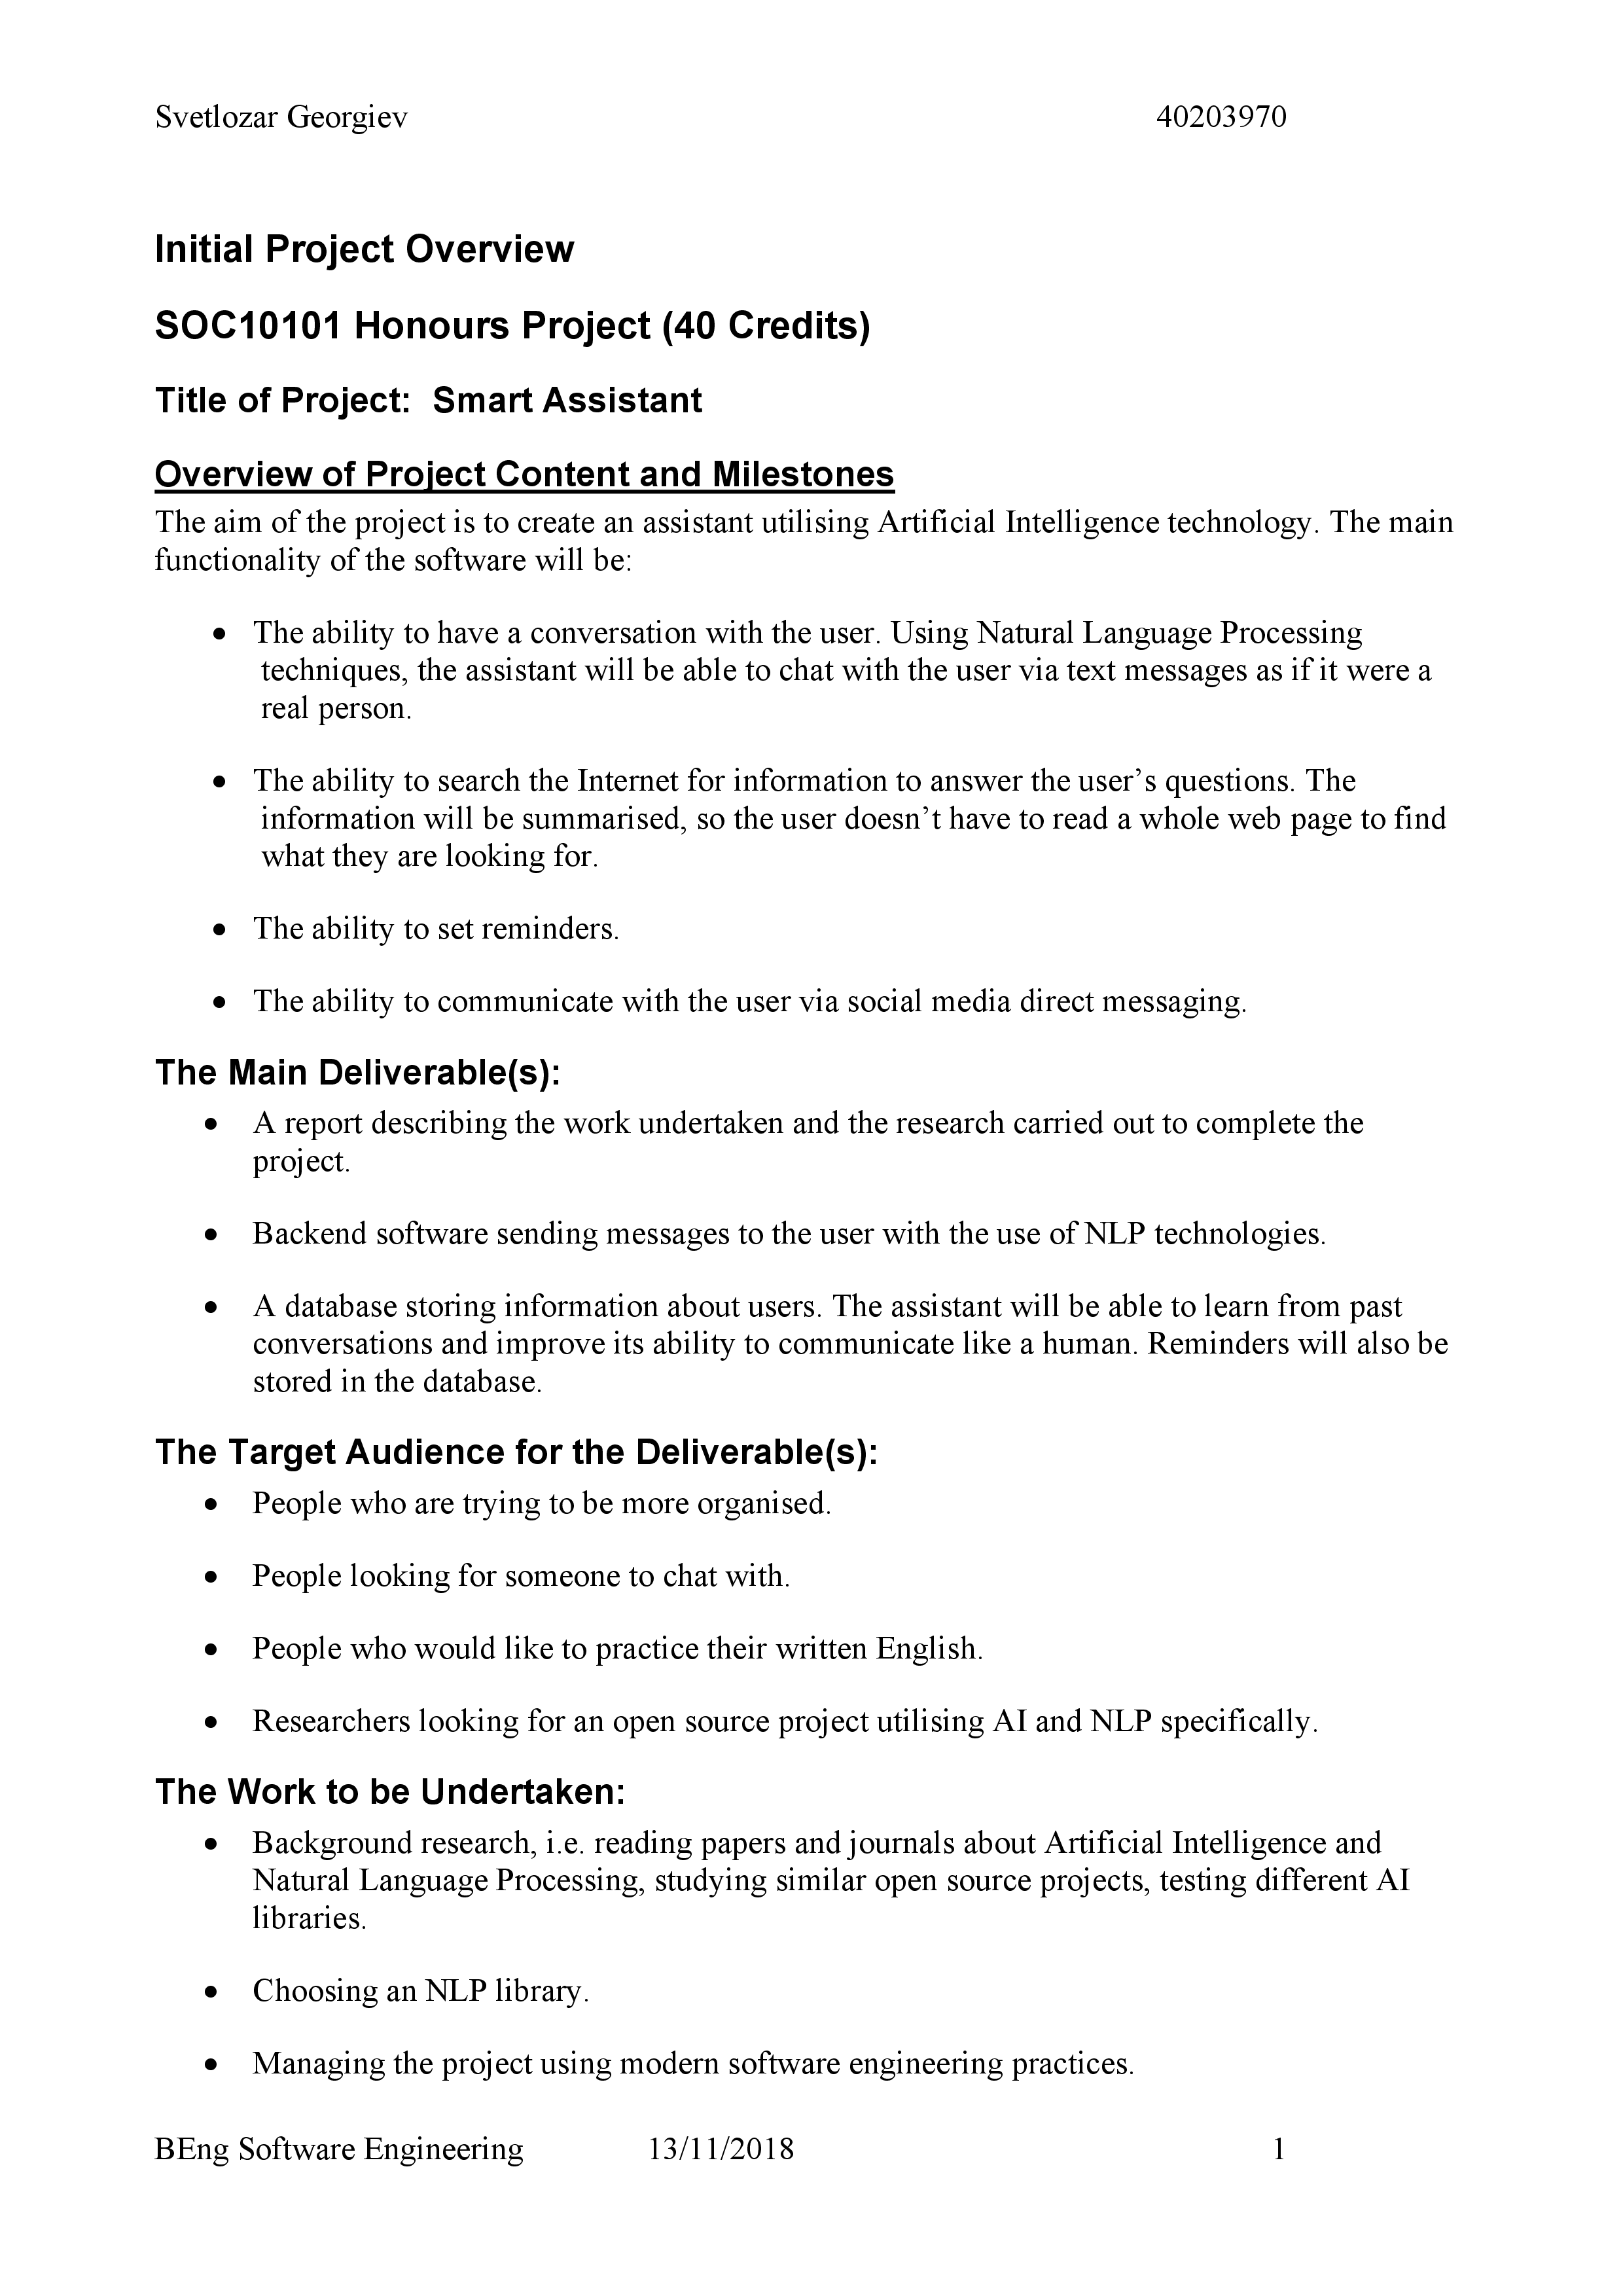
\includegraphics[width=\textwidth,height=\textheight,keepaspectratio]{IPO-0.png} % fit images to page
\newpage
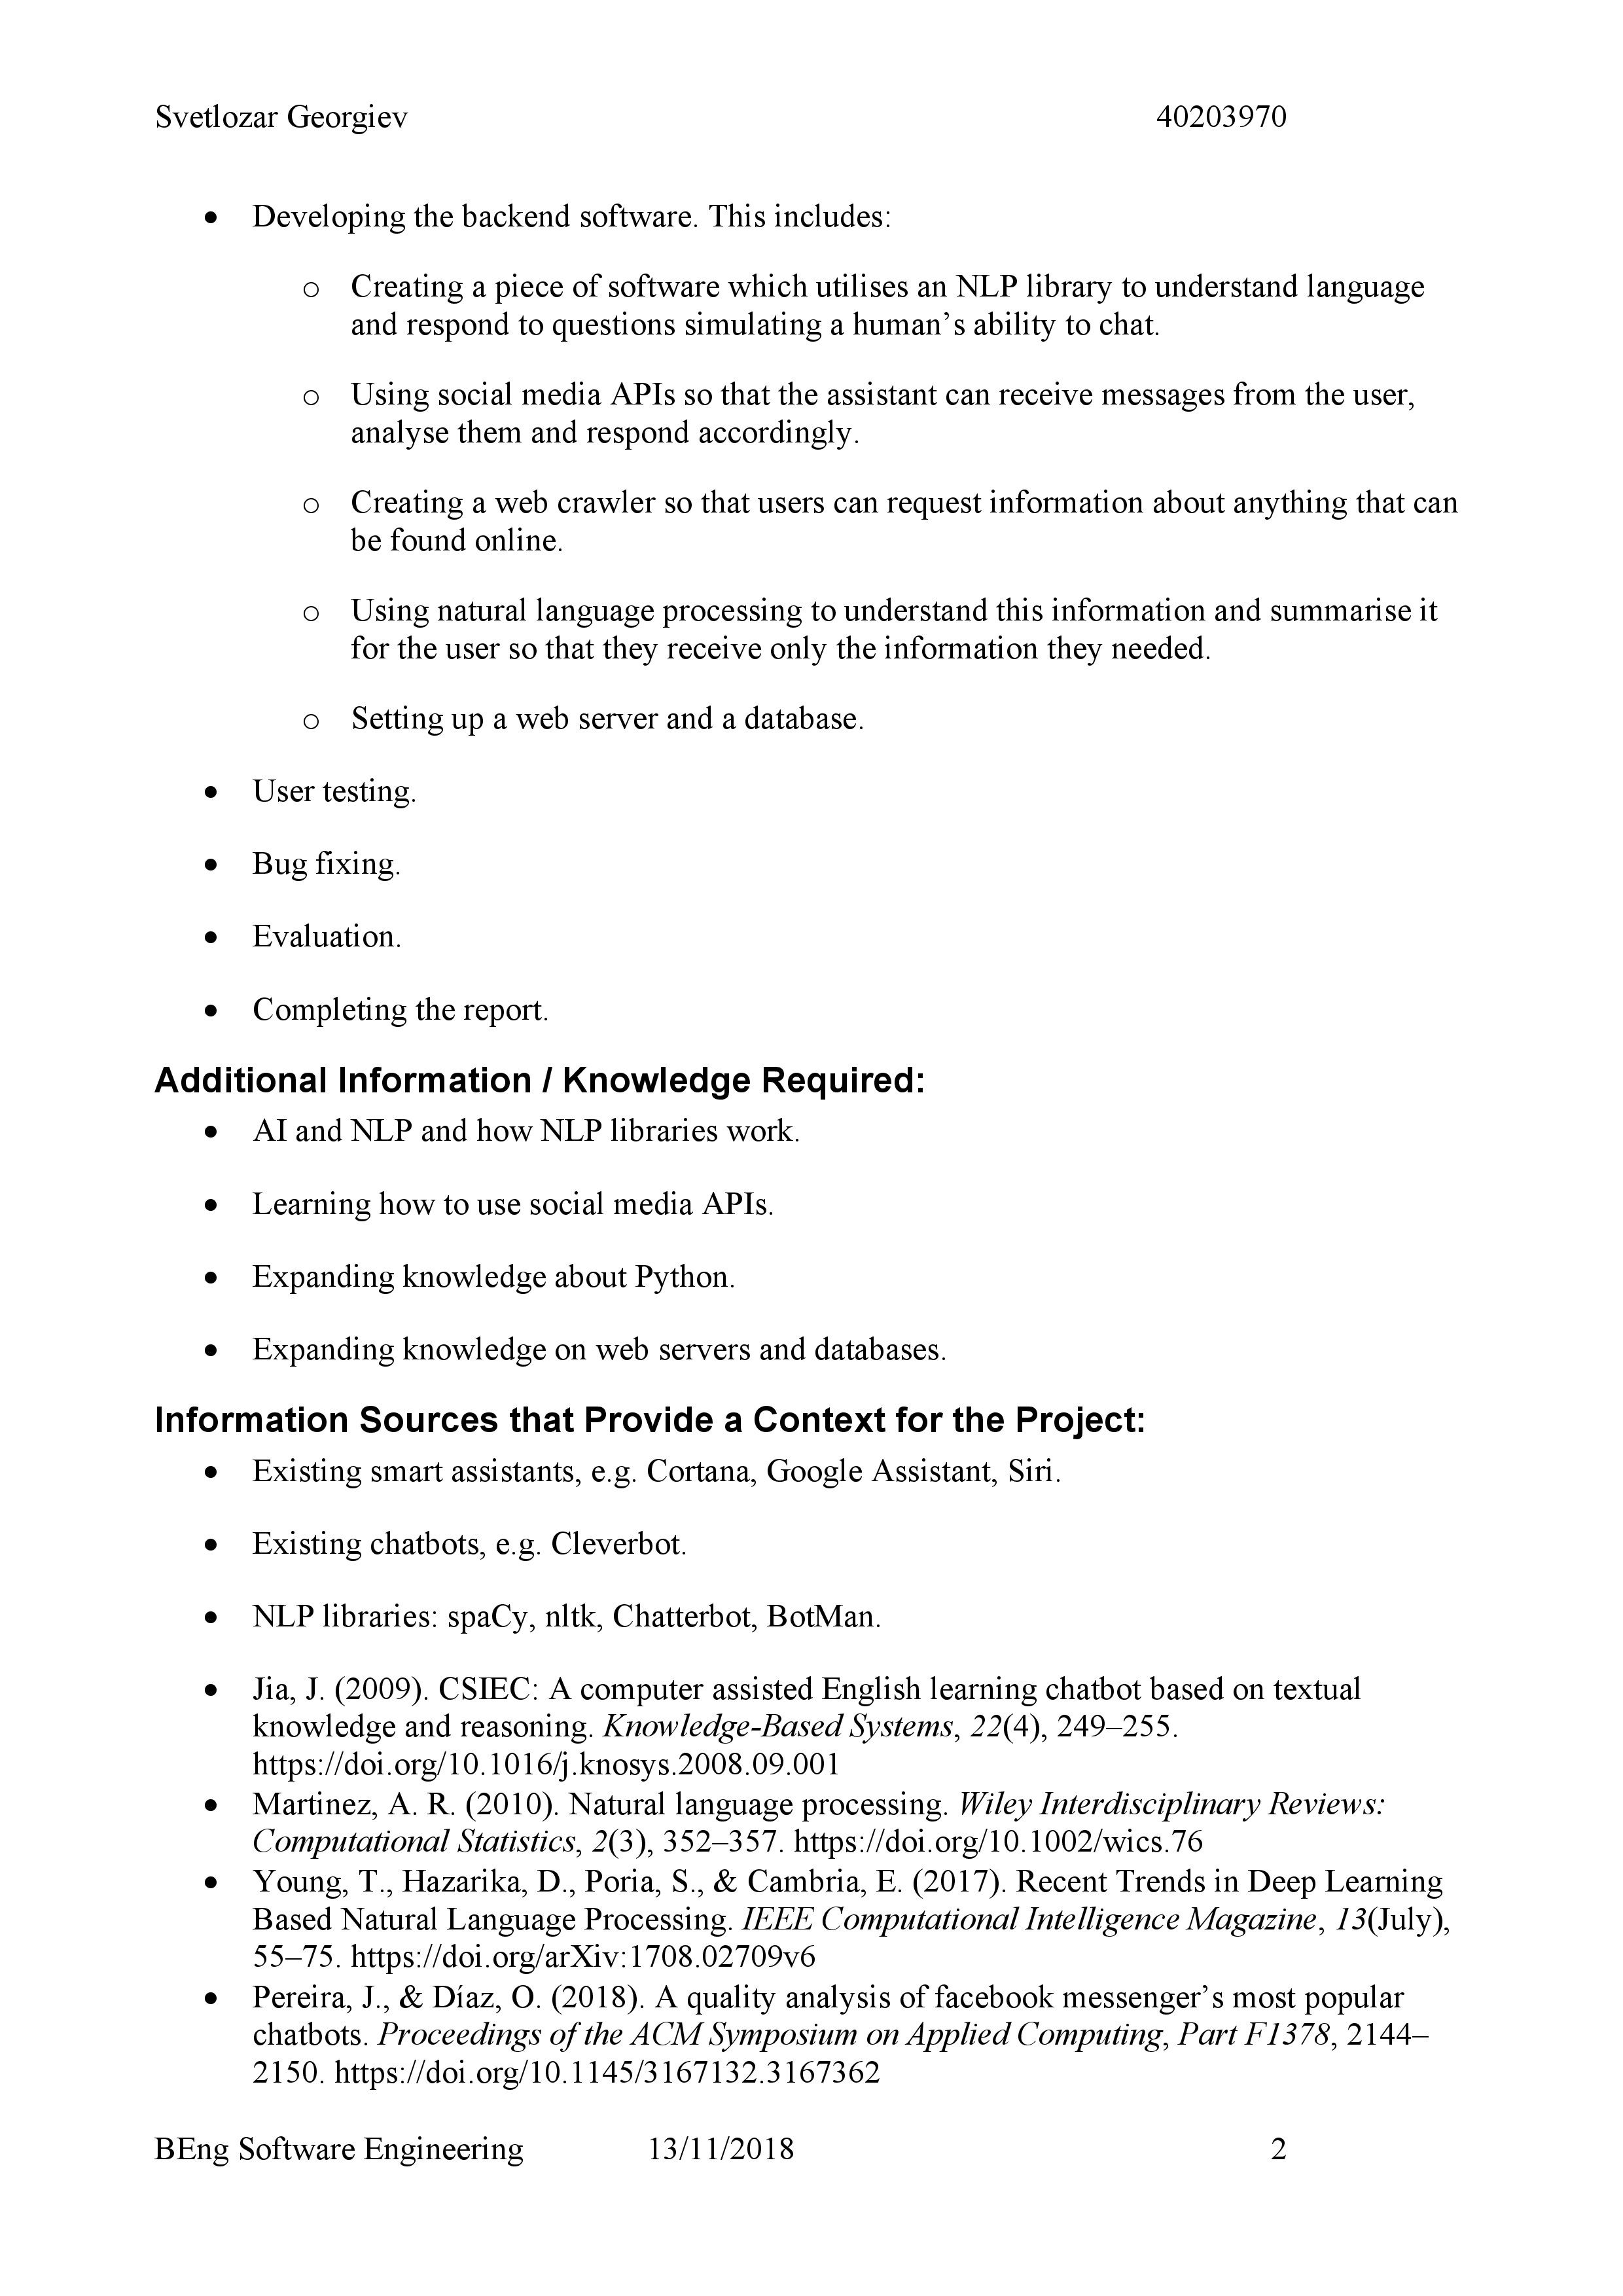
\includegraphics[width=\textwidth,height=\textheight,keepaspectratio]{IPO-1.png}
\newpage
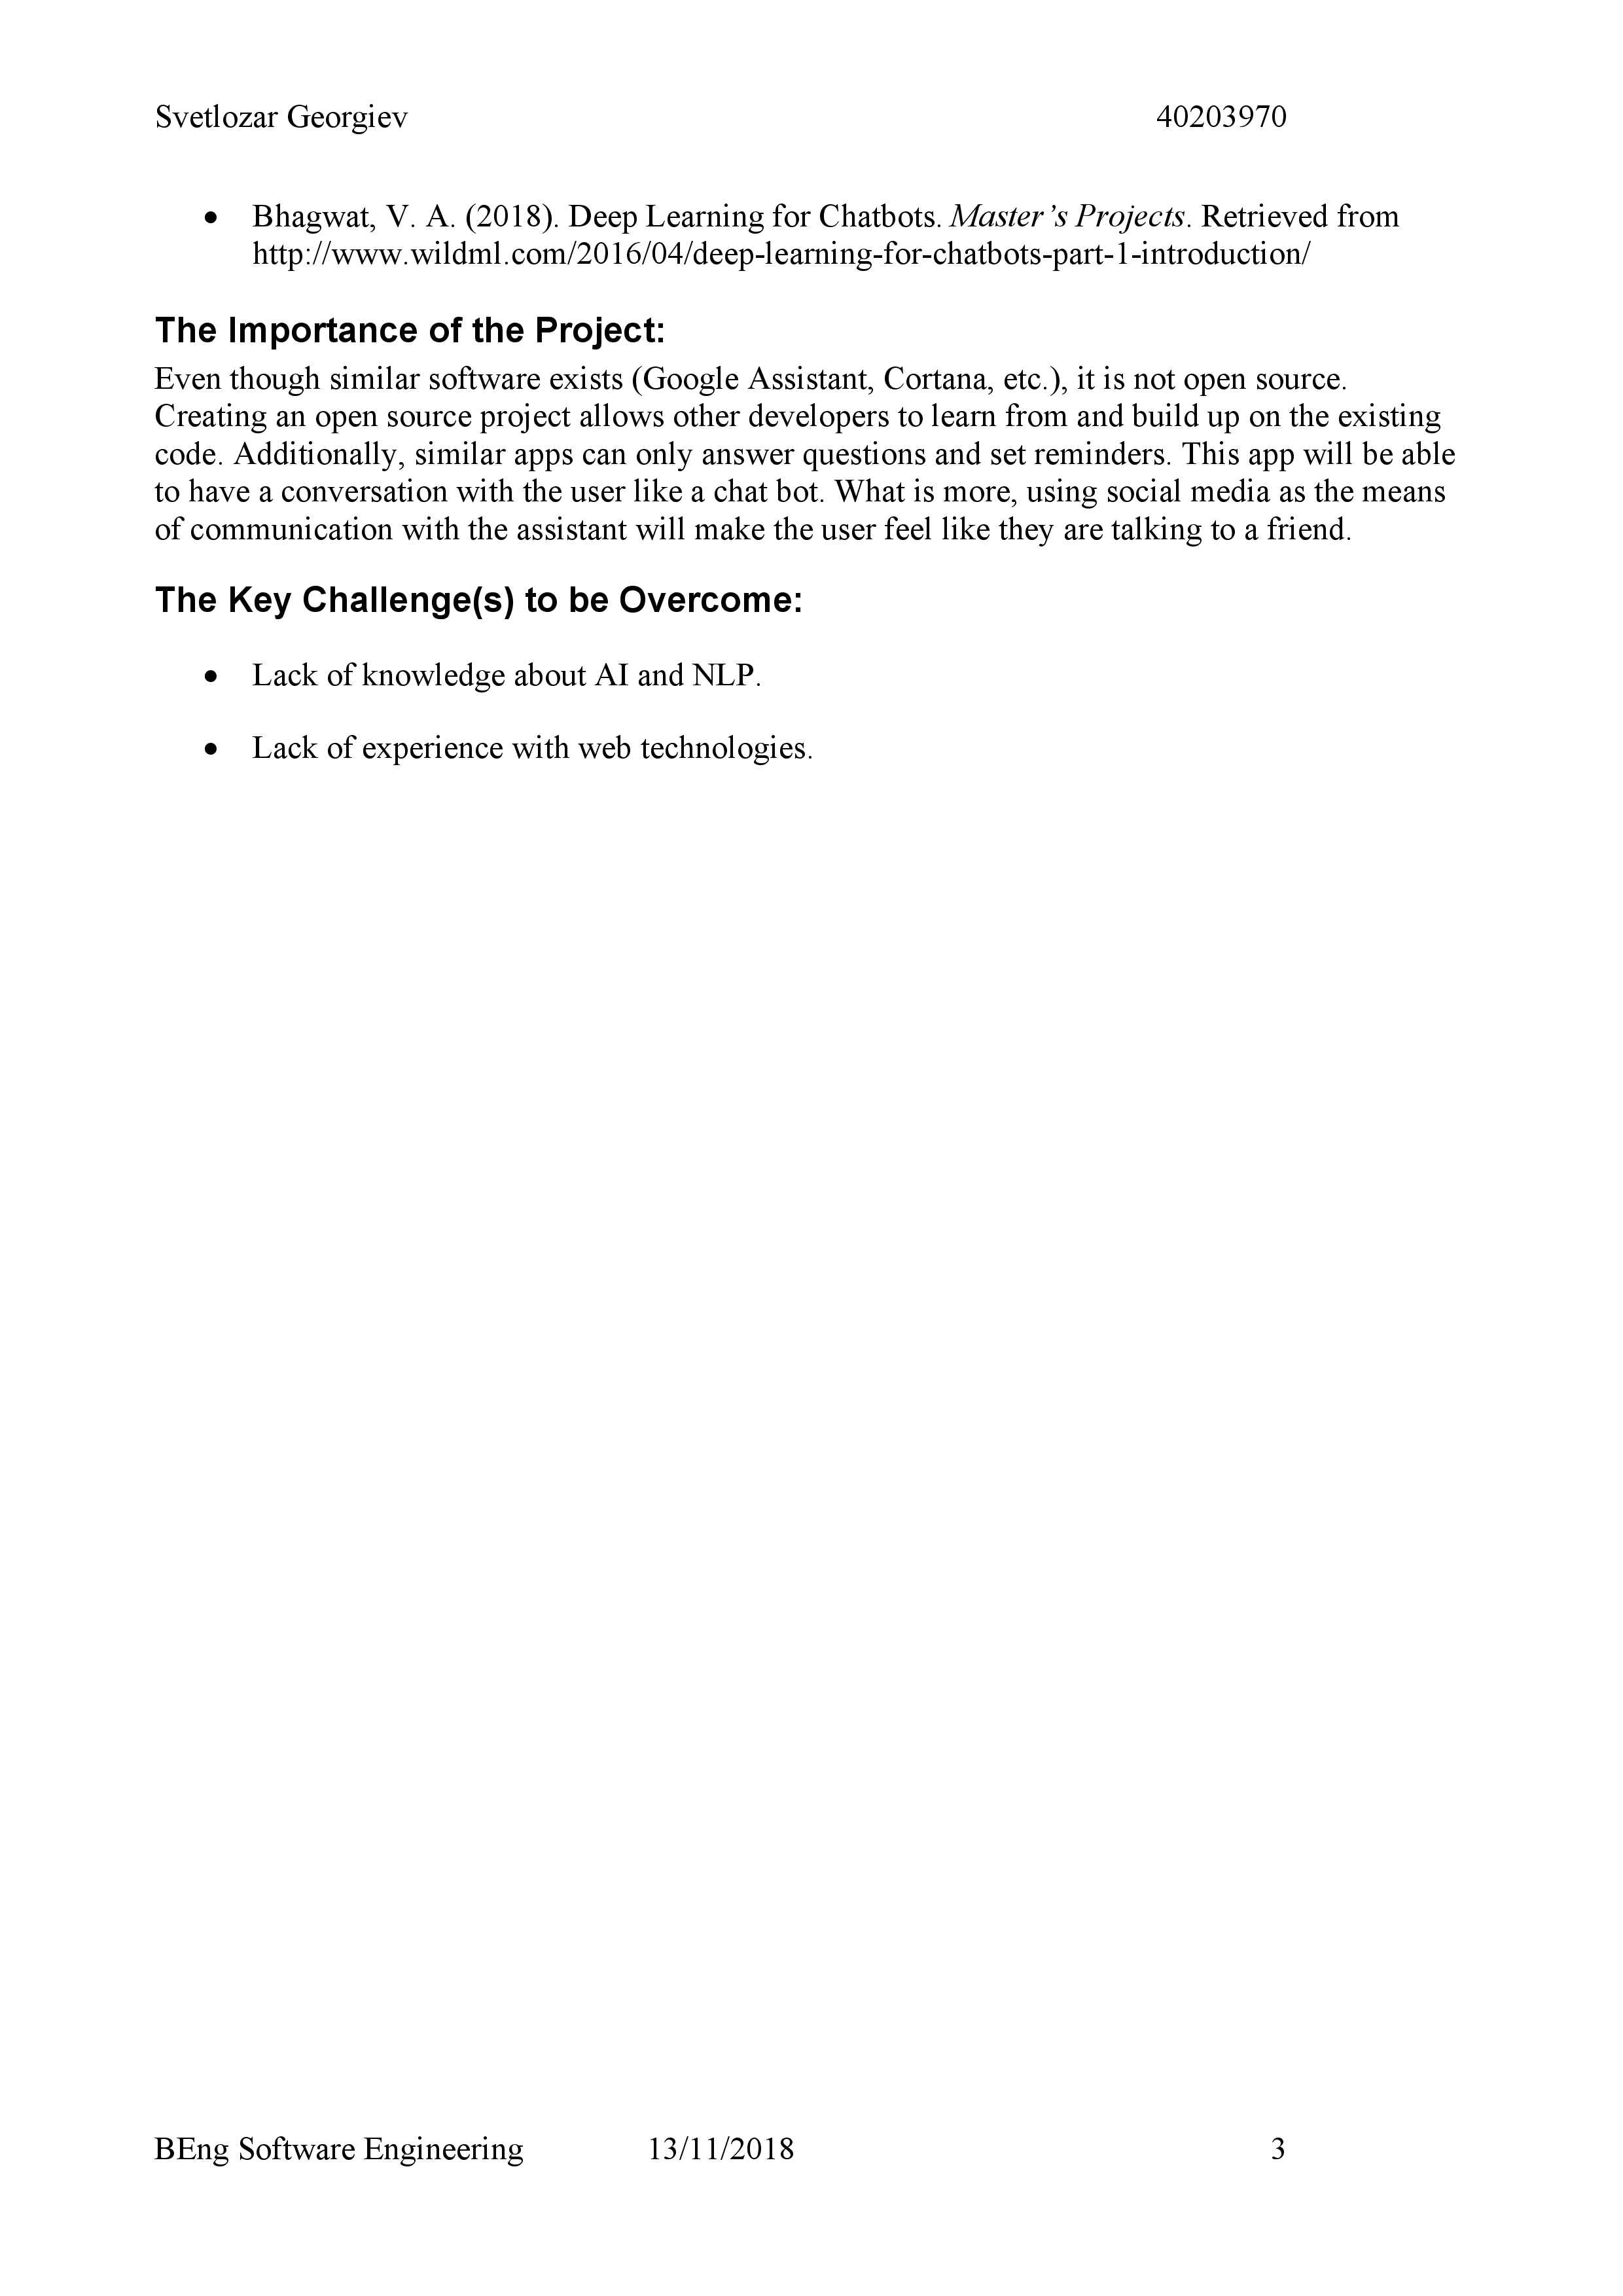
\includegraphics[width=\textwidth,height=\textheight,keepaspectratio]{IPO-2.png} 

\newpage
\section{Diary Sheets}
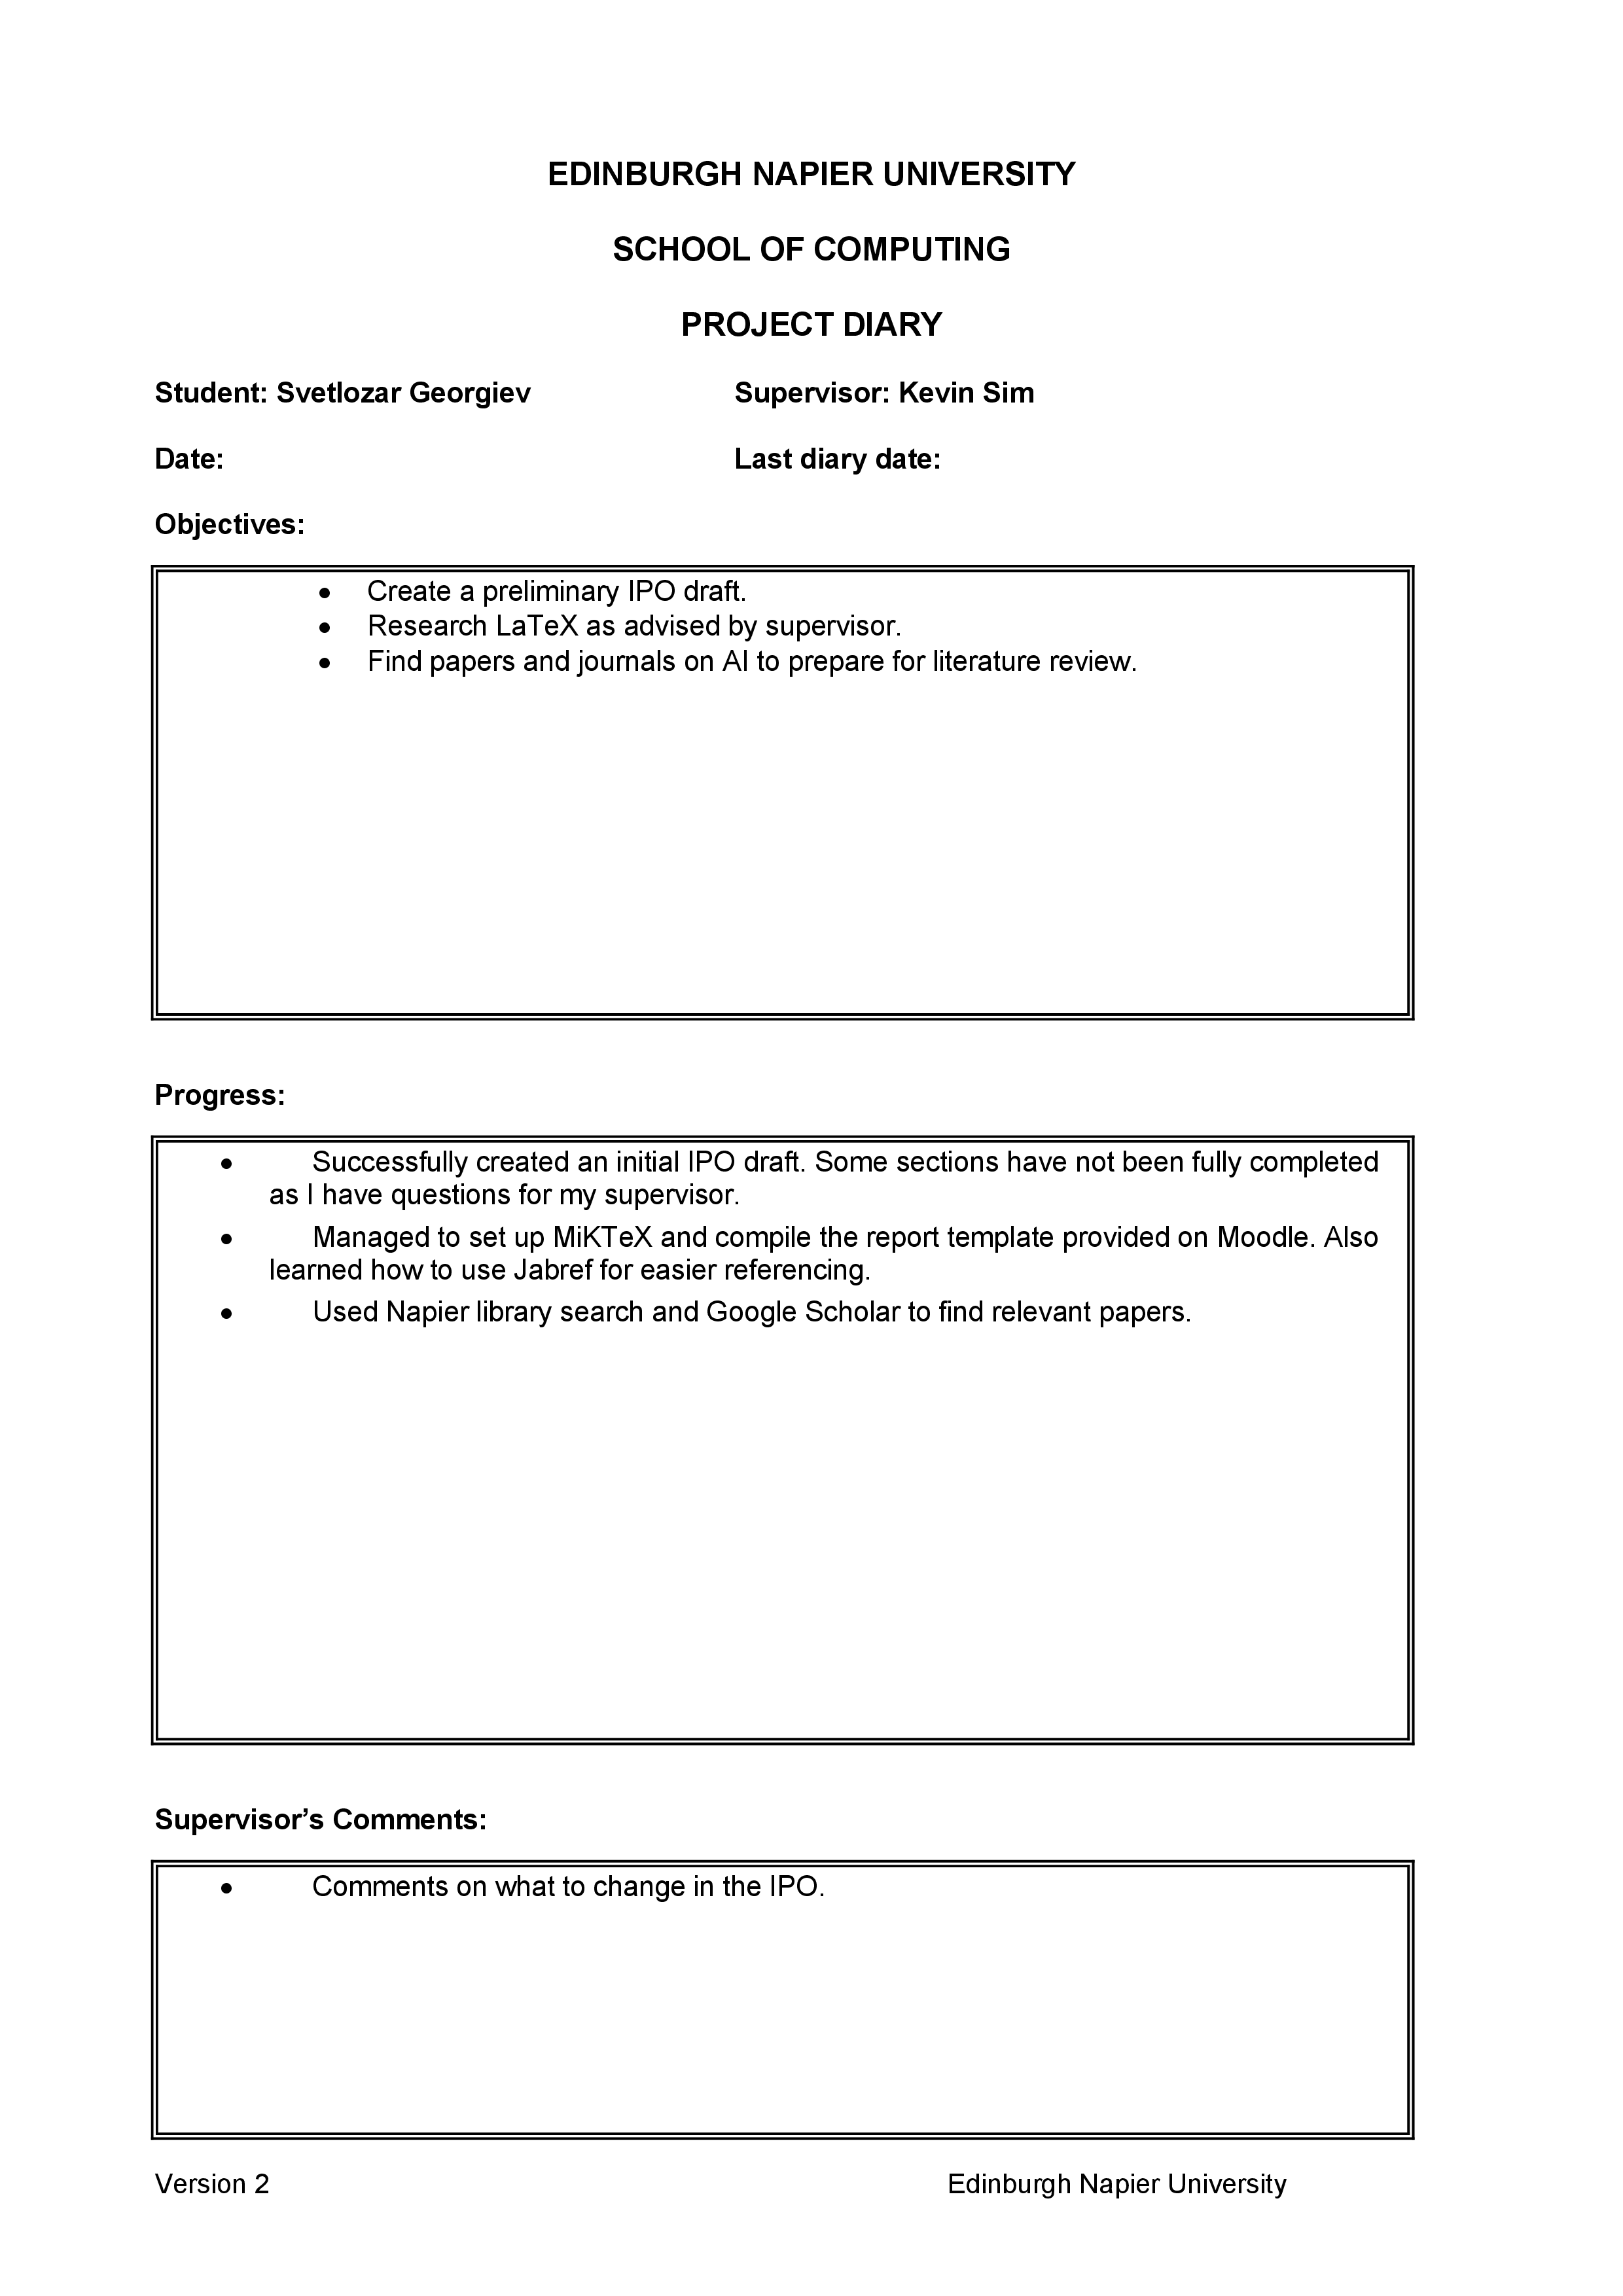
\includegraphics[width=\textwidth,height=\textheight,keepaspectratio]{diary1.png} % fit images to page
\newpage
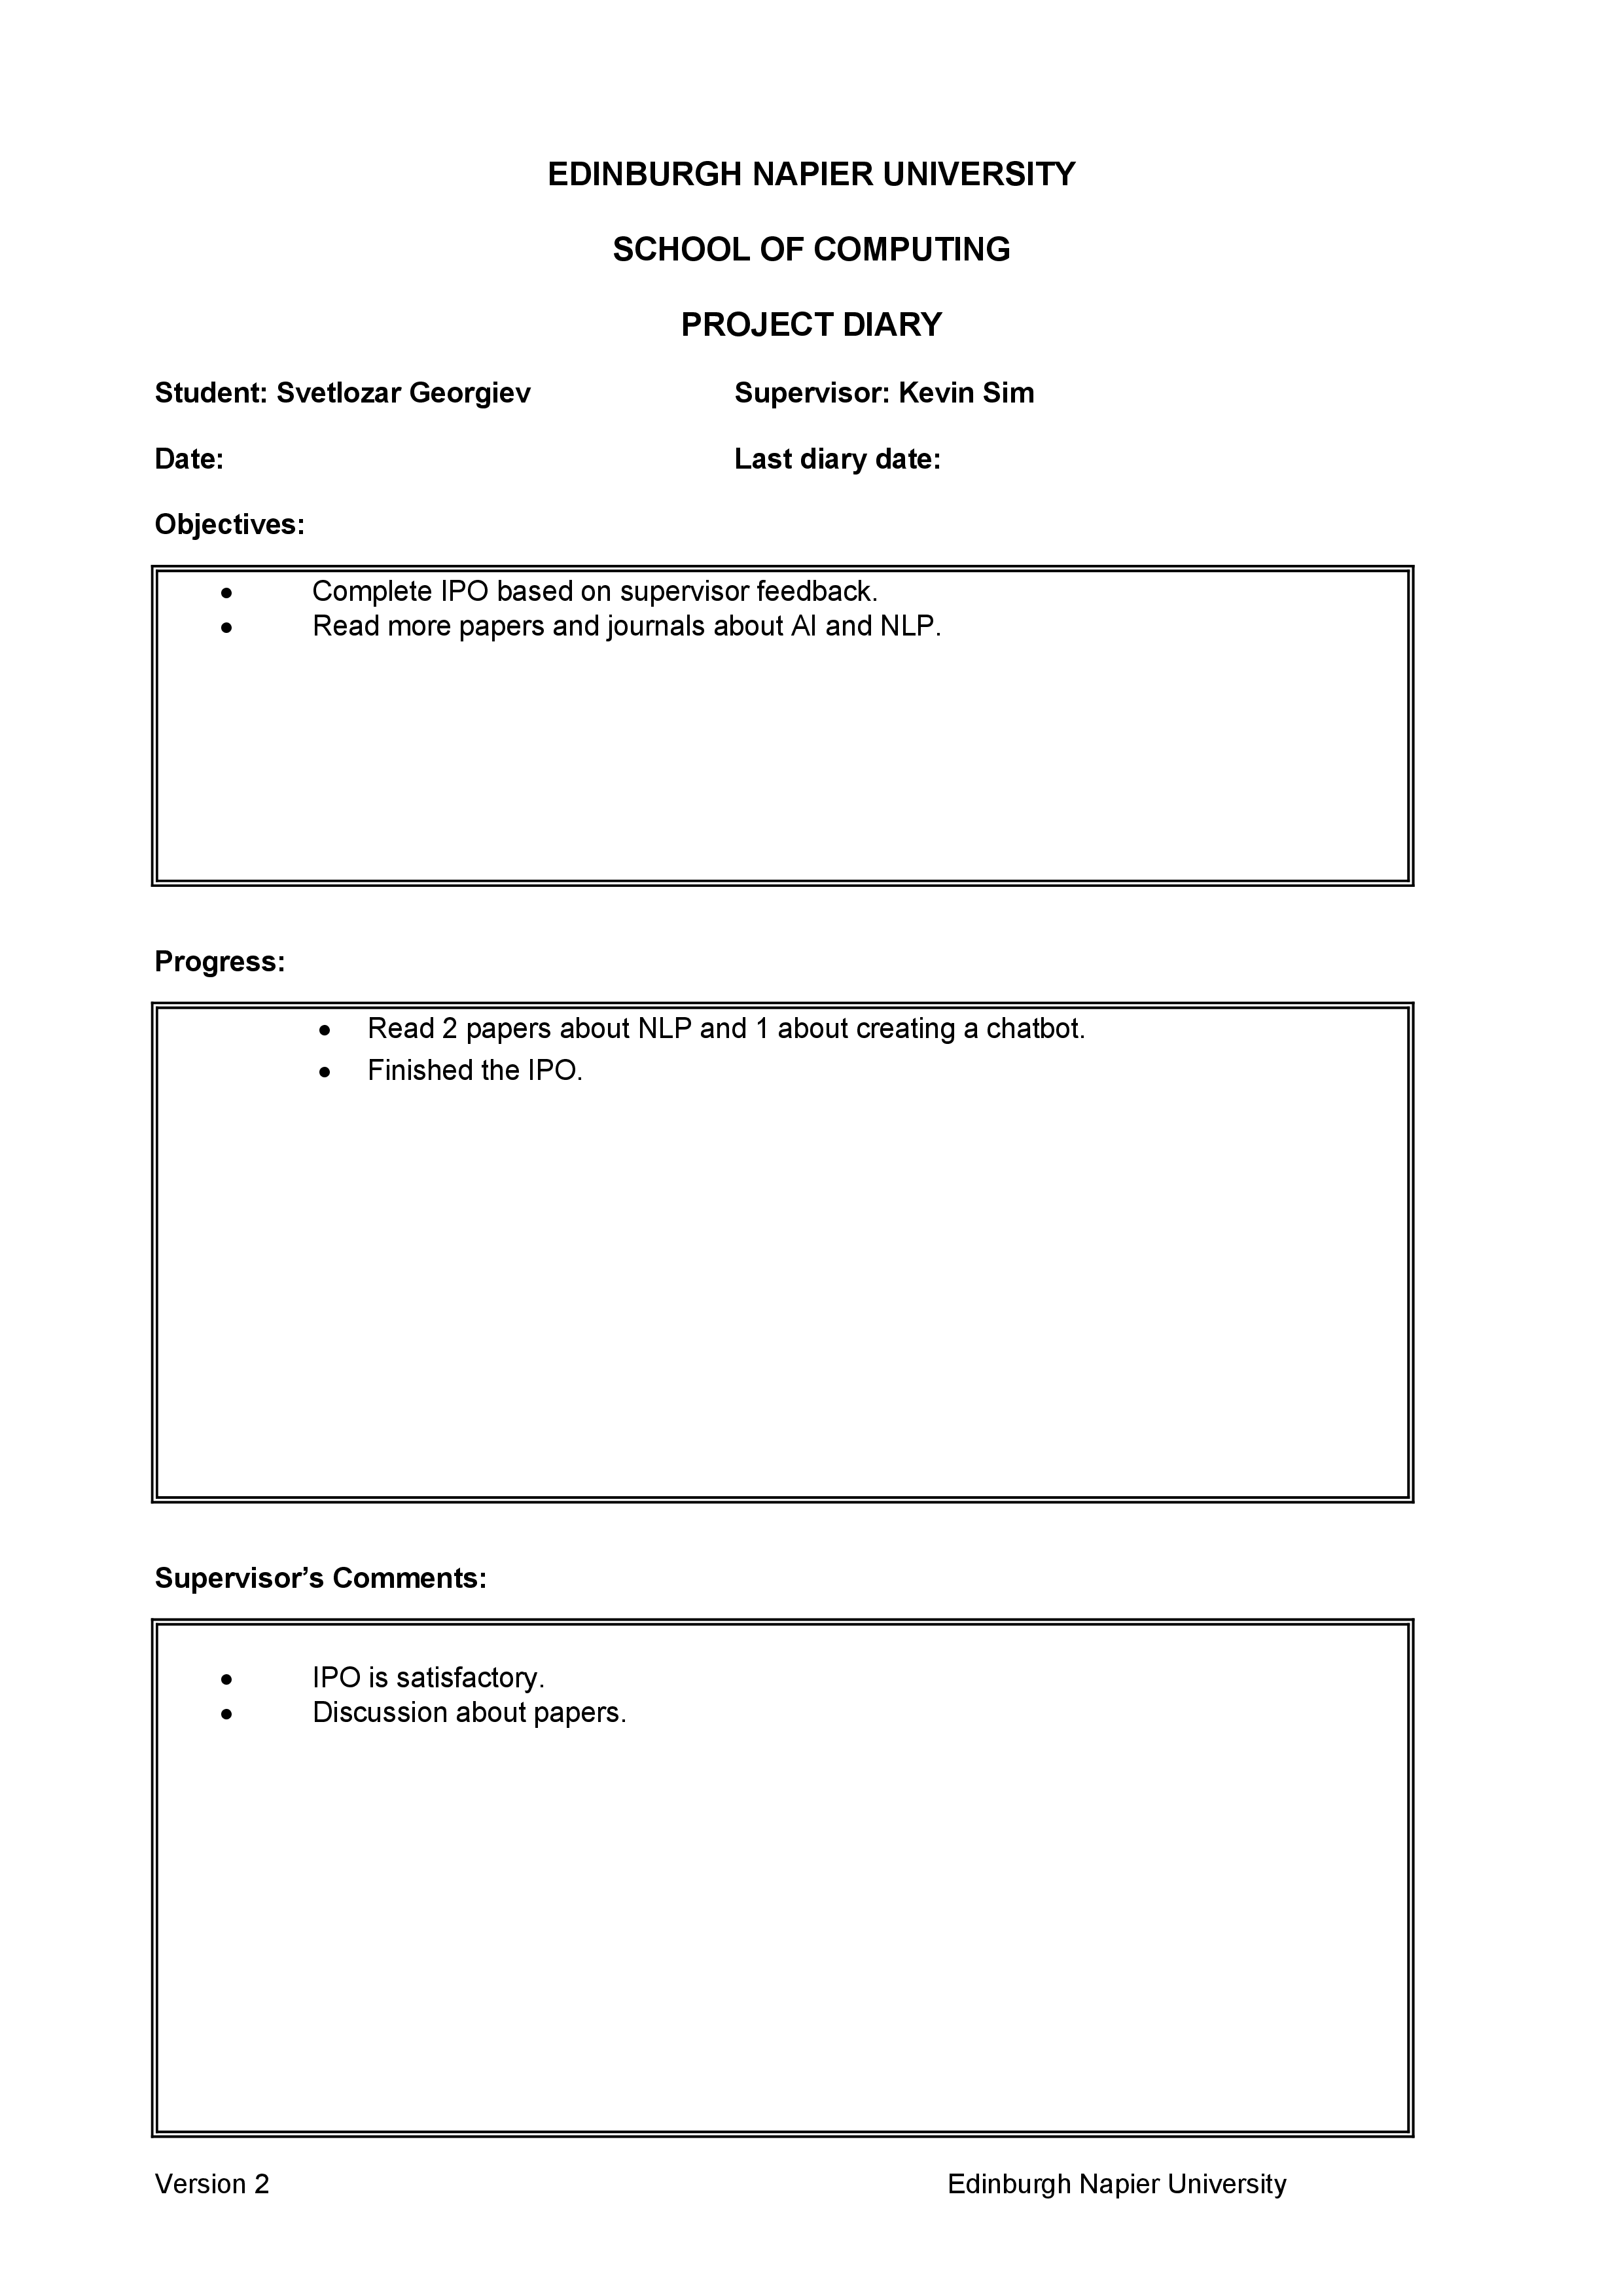
\includegraphics[width=\textwidth,height=\textheight,keepaspectratio]{diary2.png}
\newpage
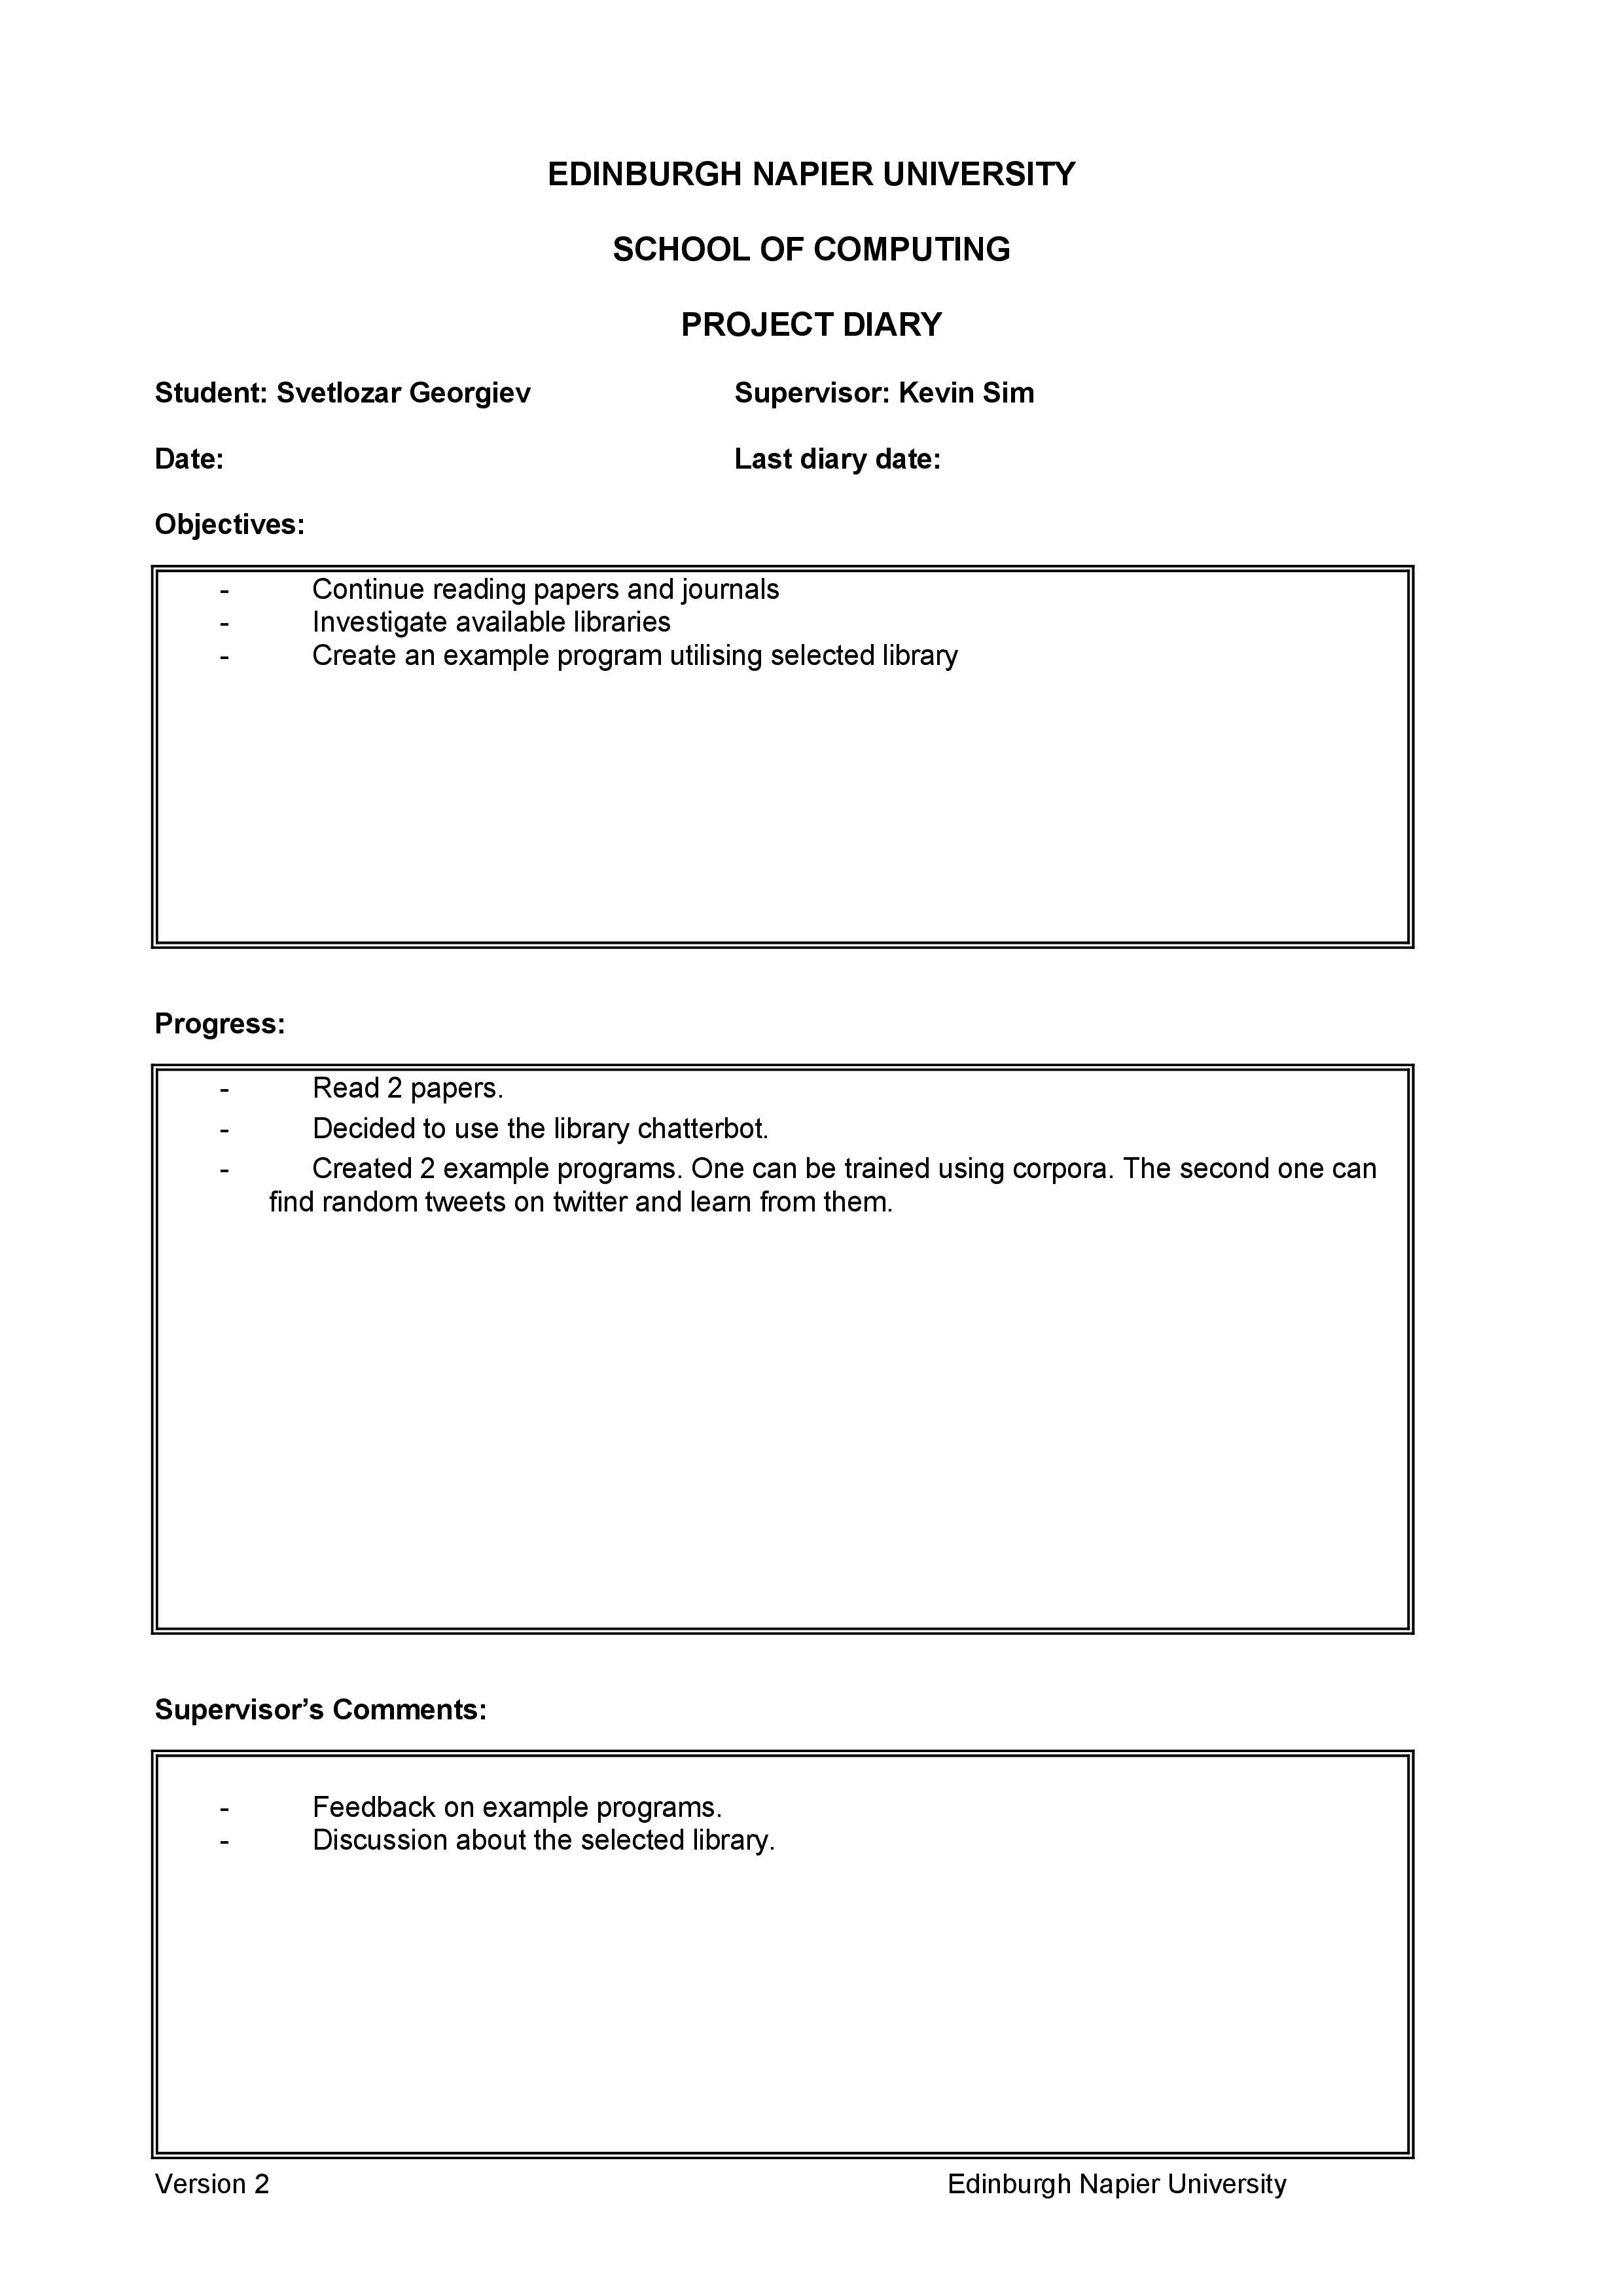
\includegraphics[width=\textwidth,height=\textheight,keepaspectratio]{diary3.png} 
\newpage
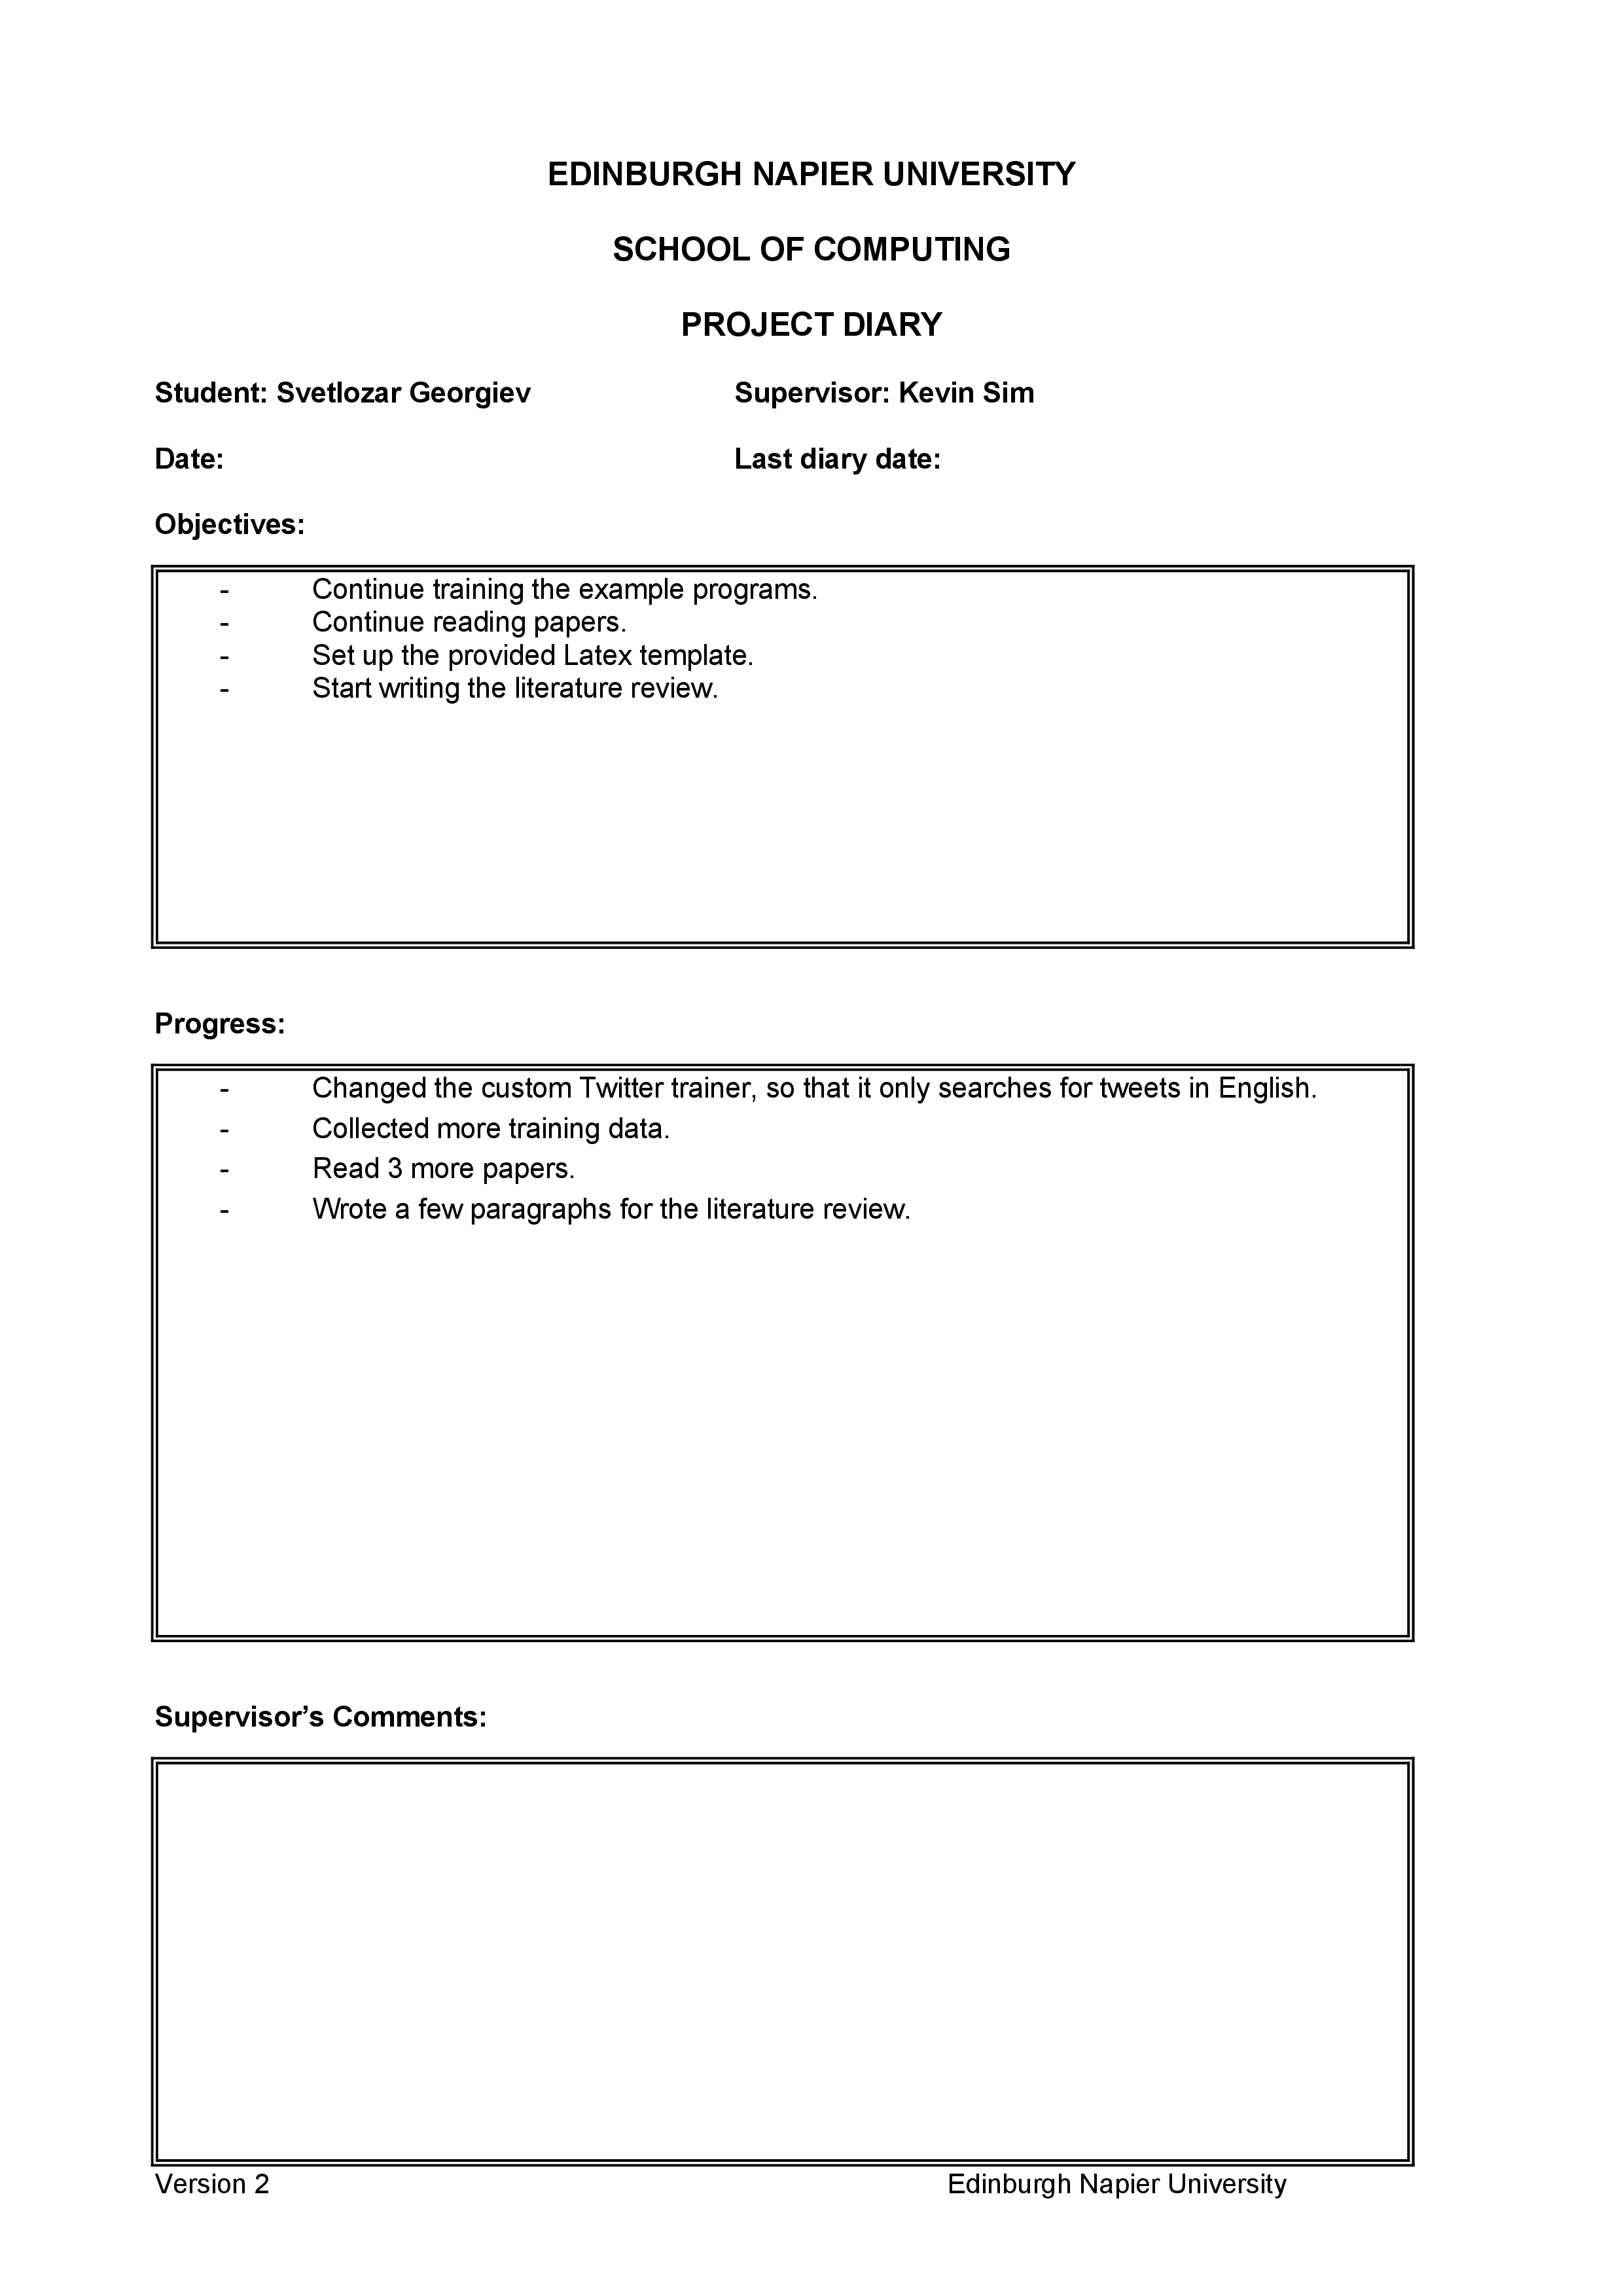
\includegraphics[width=\textwidth,height=\textheight,keepaspectratio]{diary4.png} 
\newpage
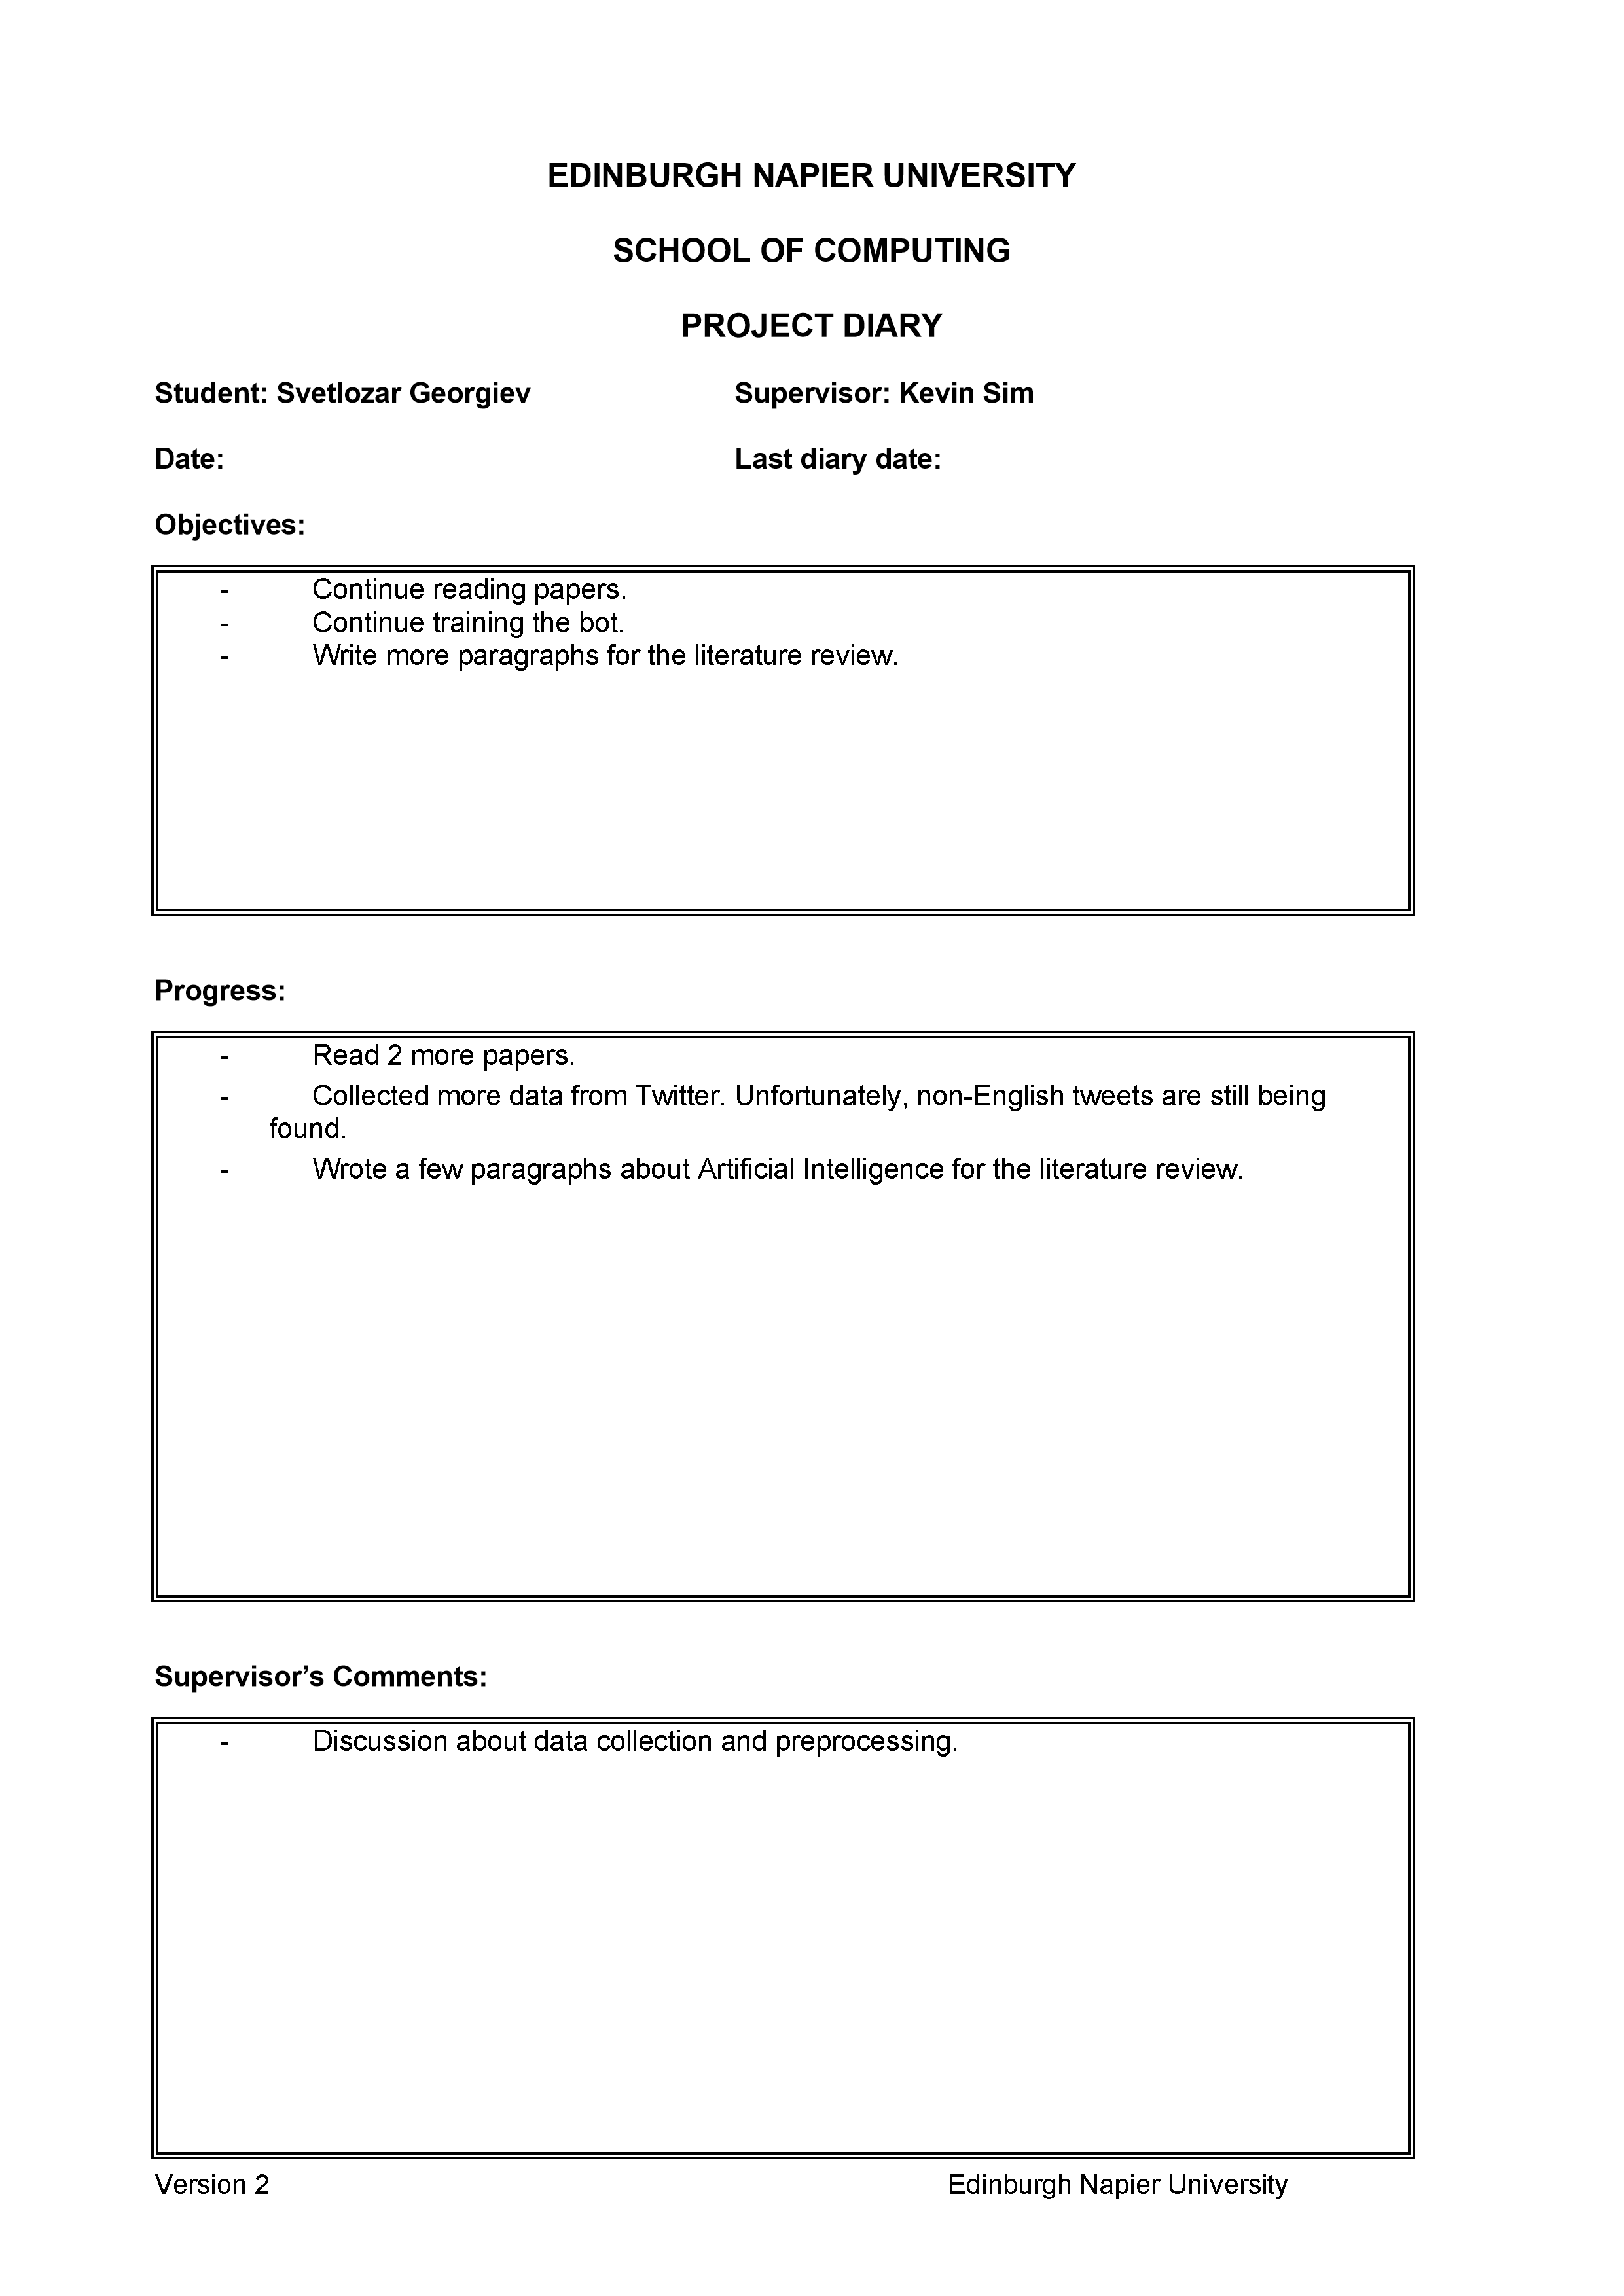
\includegraphics[width=\textwidth,height=\textheight,keepaspectratio]{diary5.png} 
\newpage
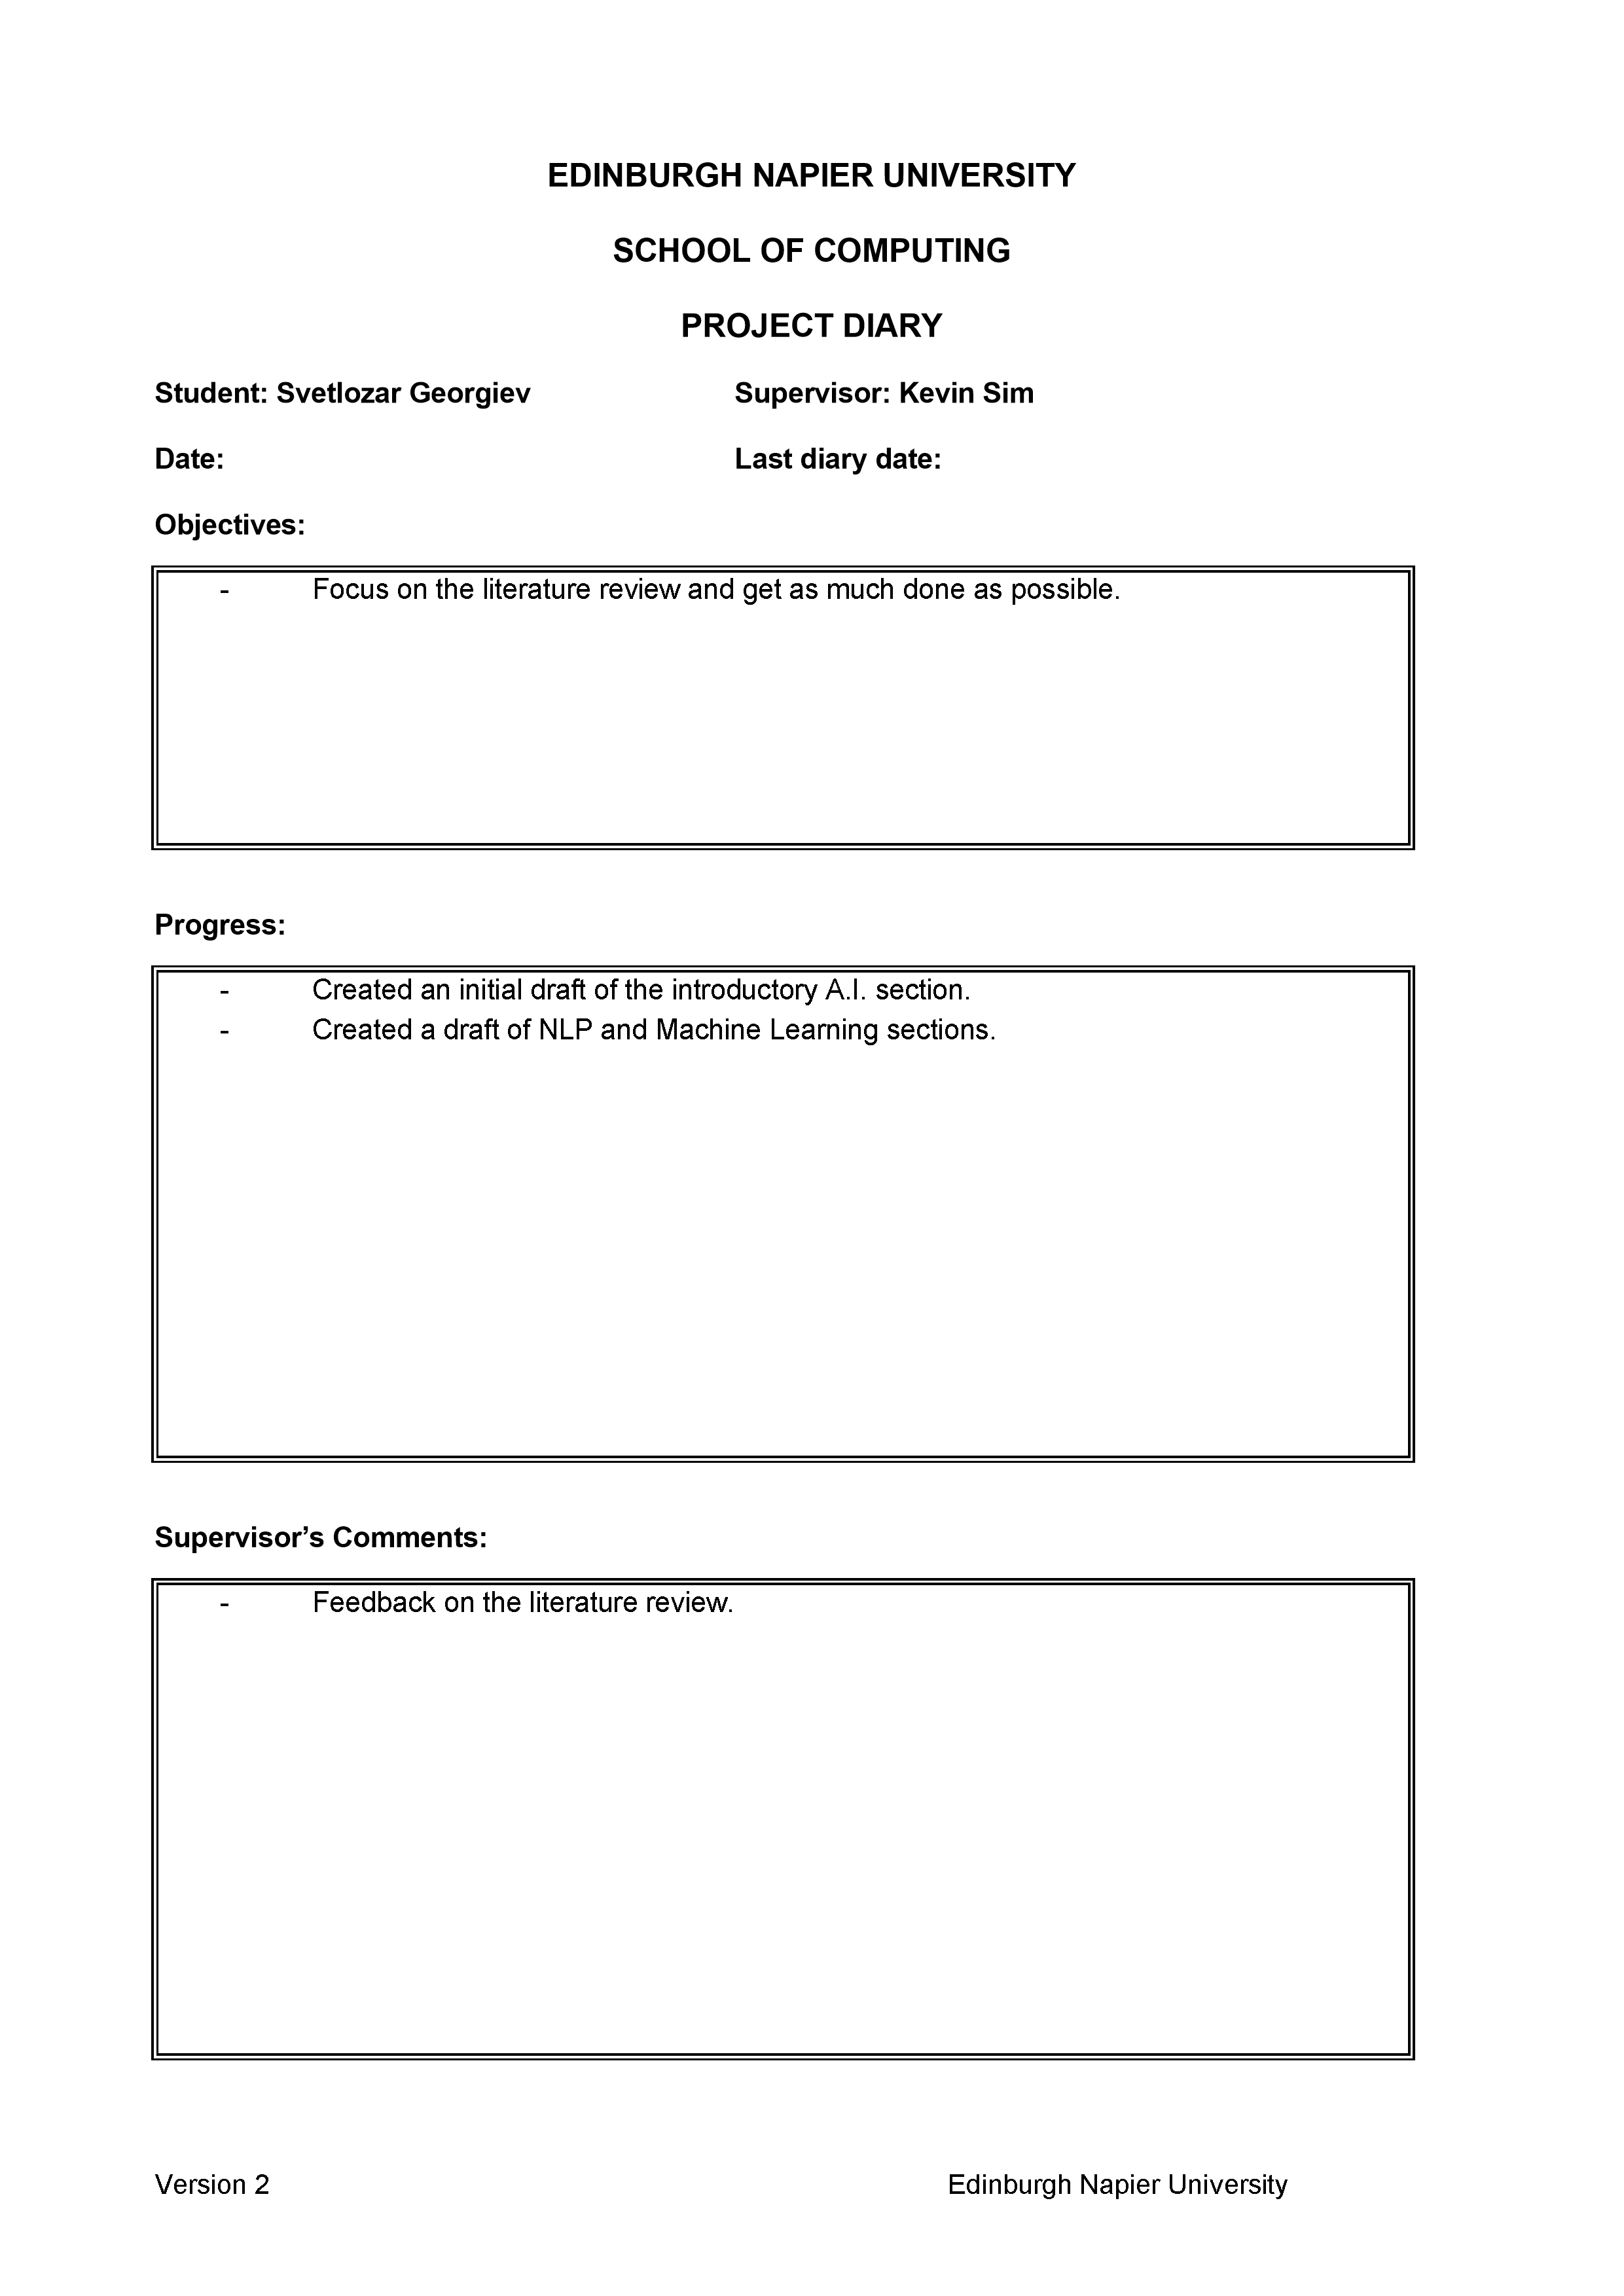
\includegraphics[width=\textwidth,height=\textheight,keepaspectratio]{diary6.png} 

\newpage
\section{Second Formal Review Output}
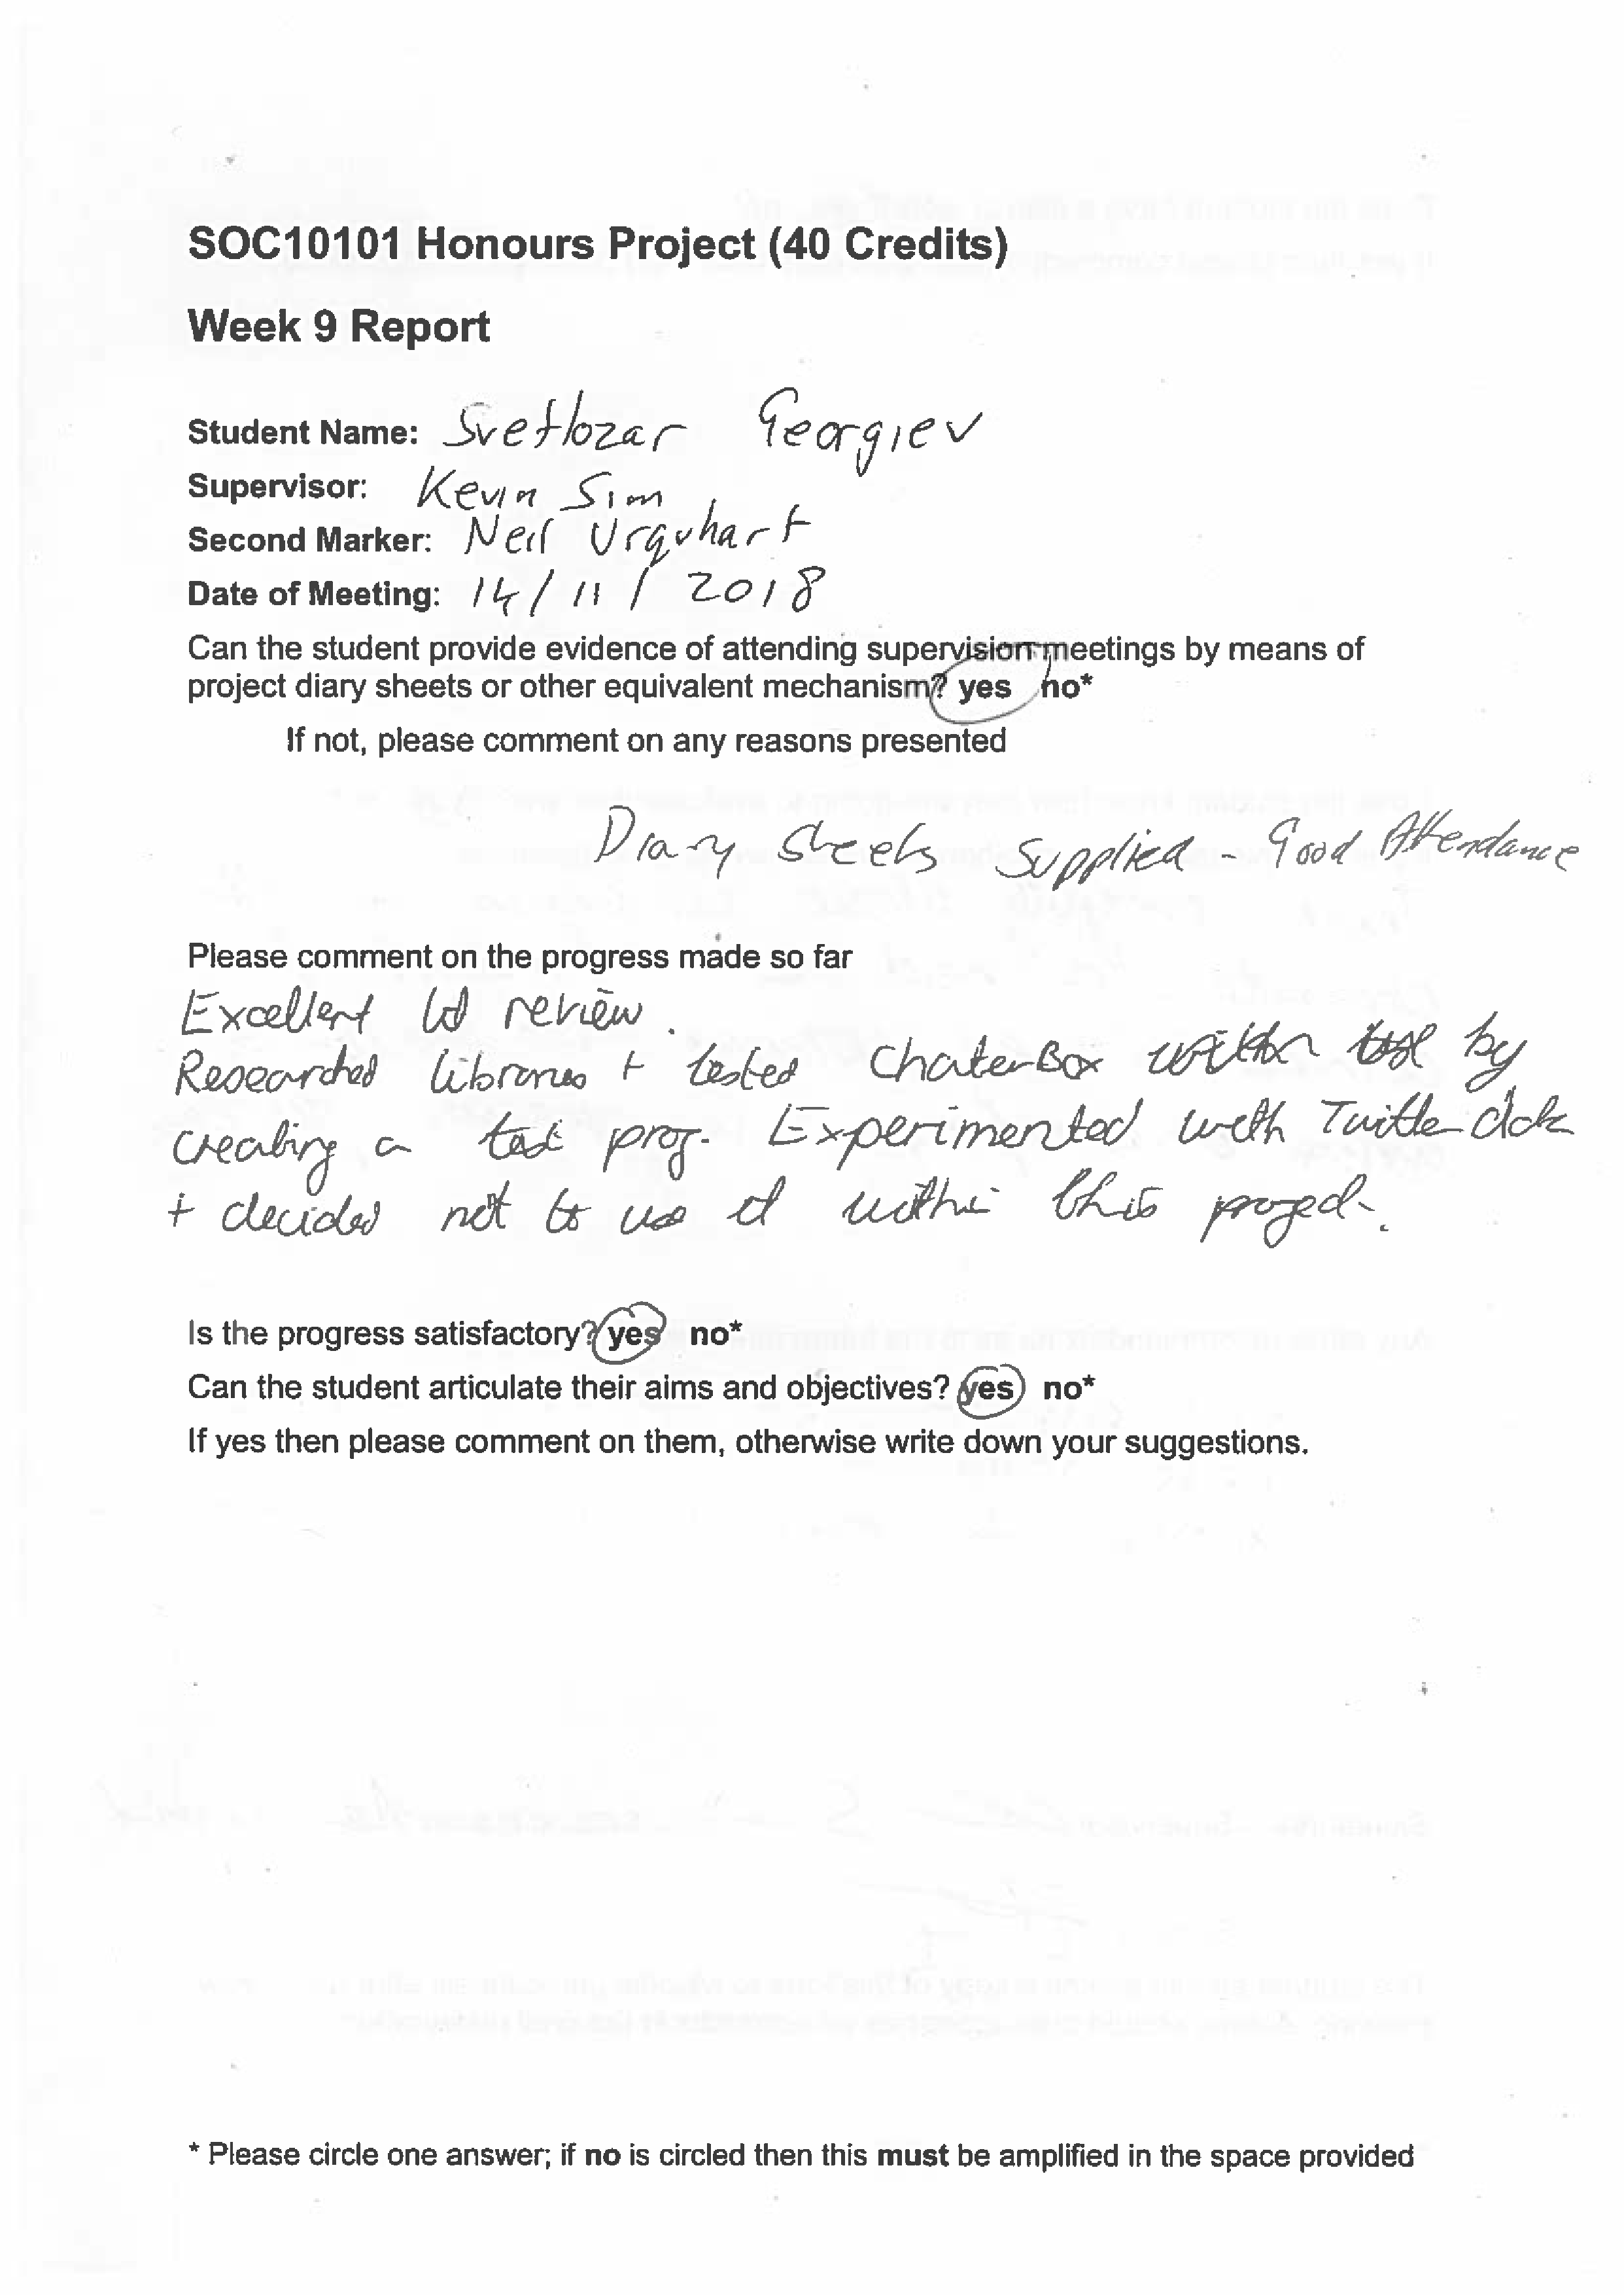
\includegraphics[width=\textwidth,height=\textheight,keepaspectratio]{interim-1.png} 
\newpage
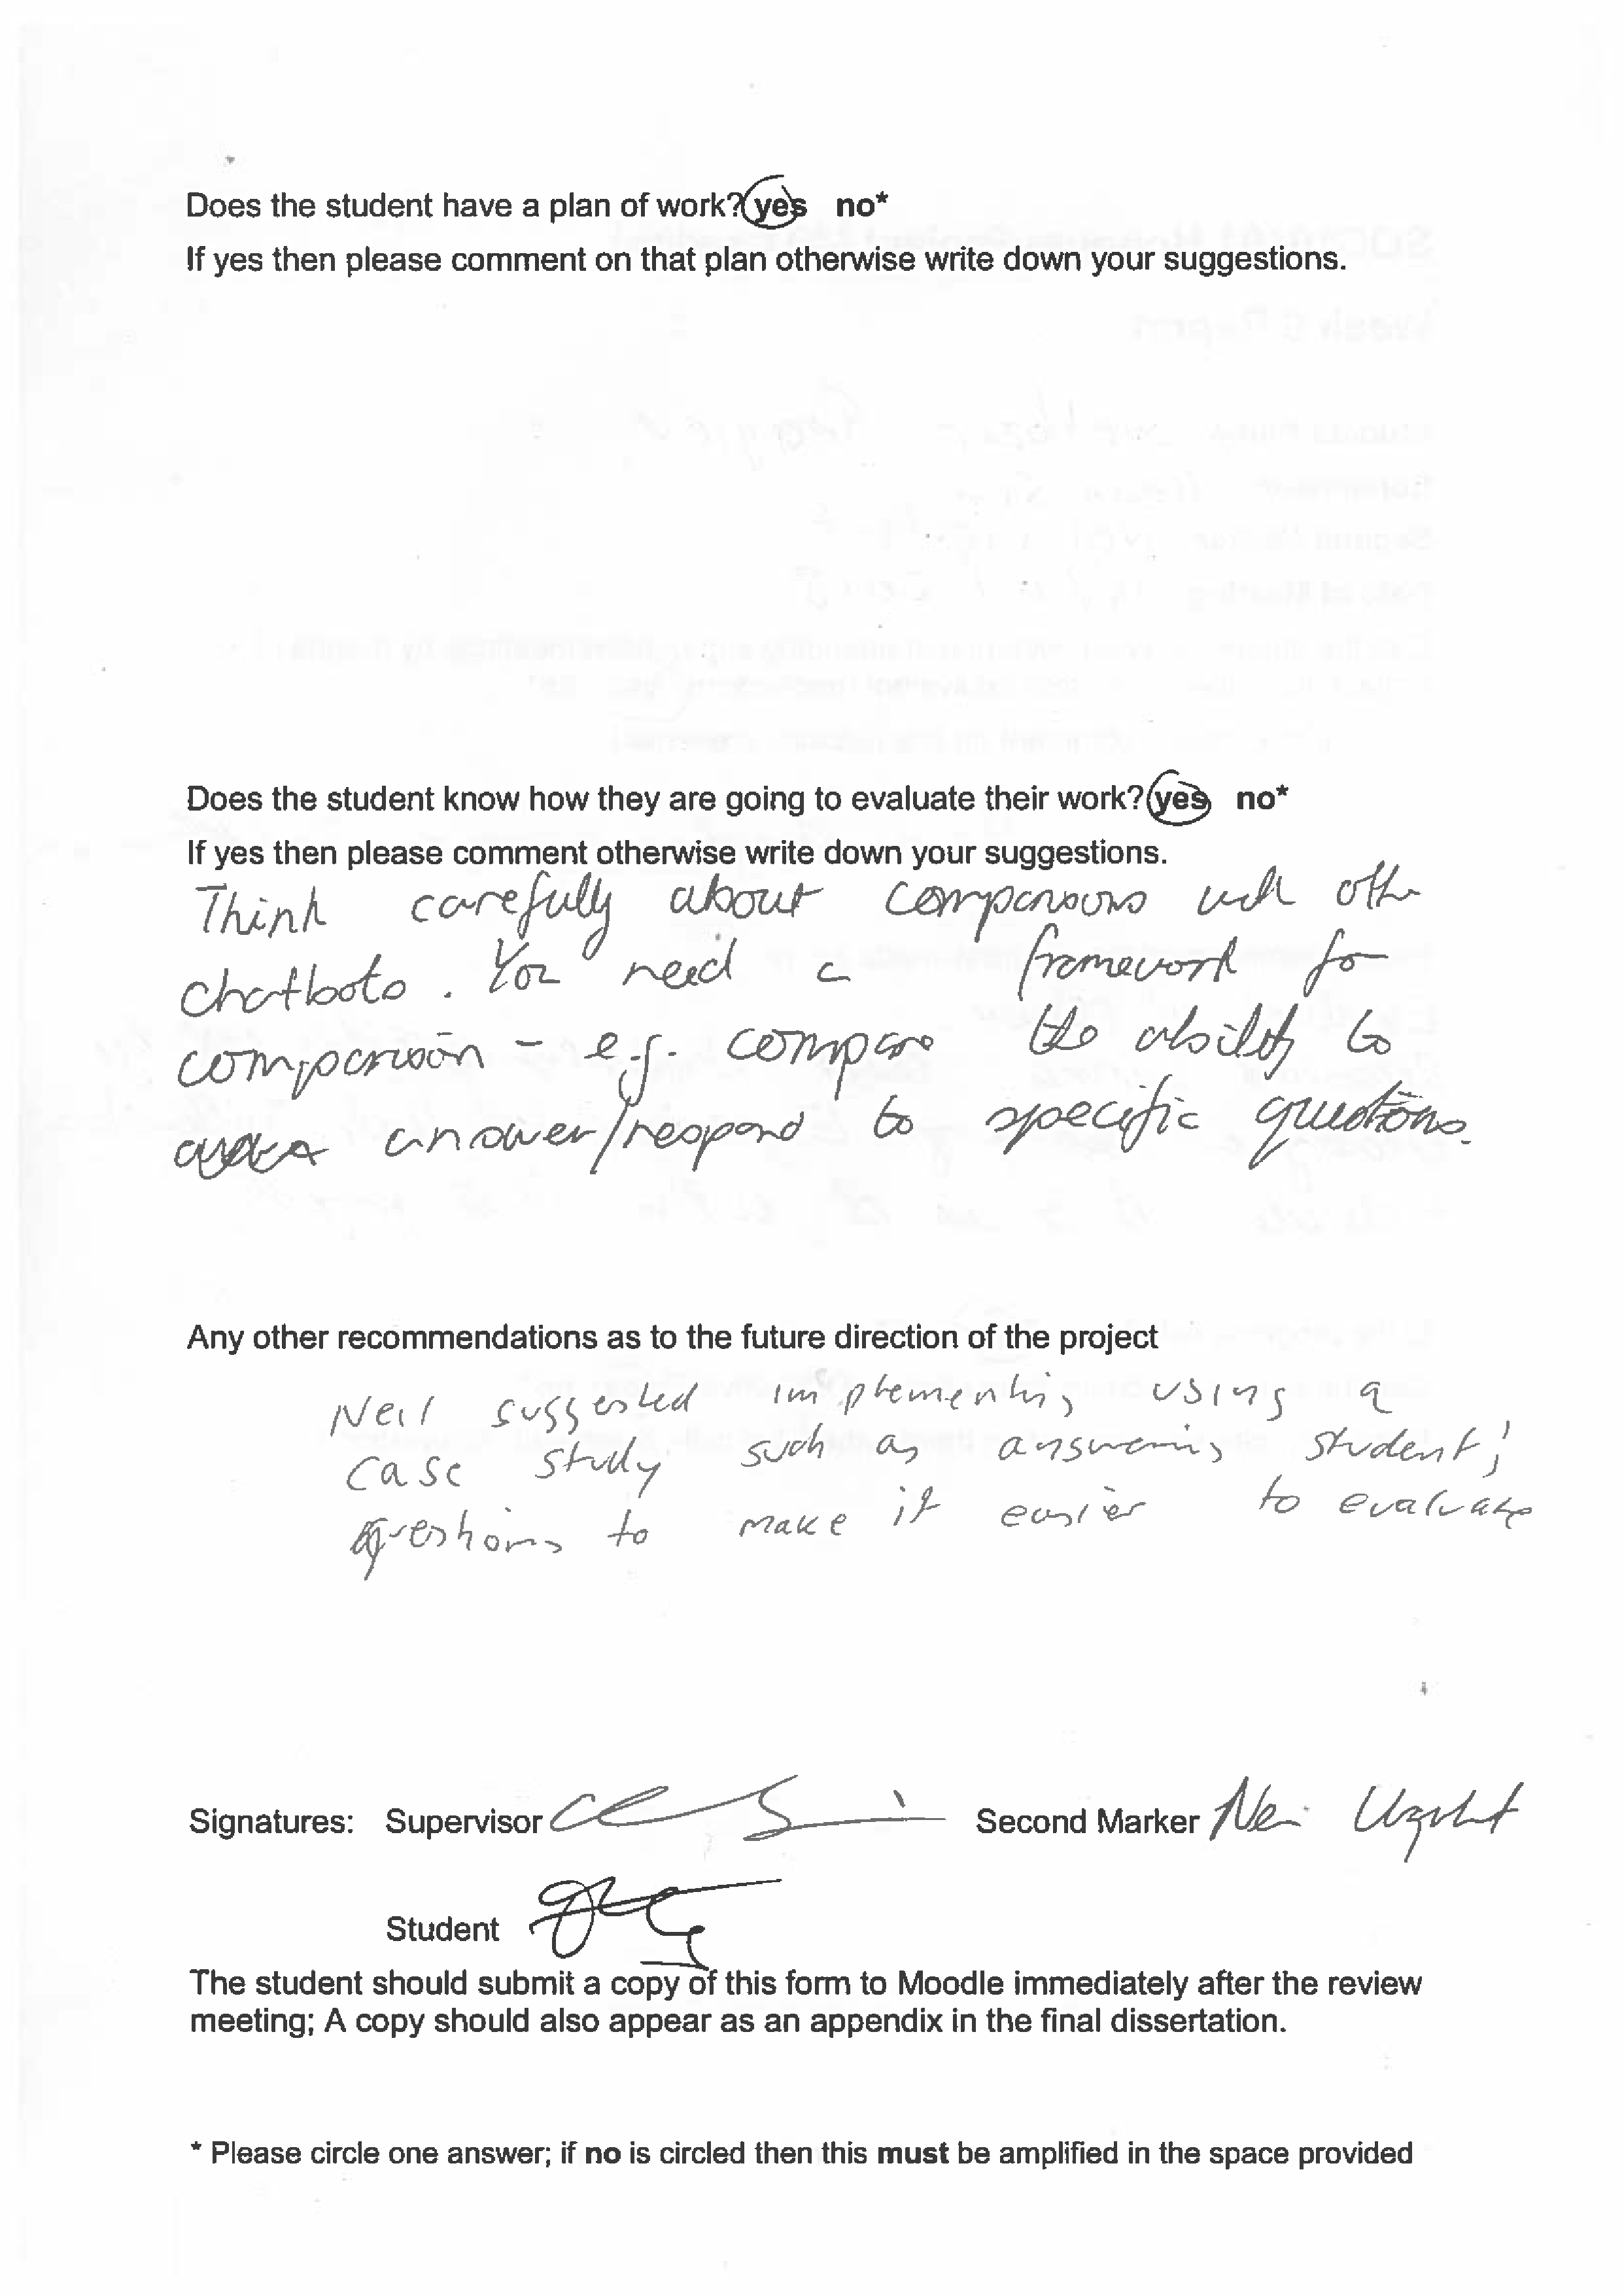
\includegraphics[width=\textwidth,height=\textheight,keepaspectratio]{interim-2.png} 

\end{appendices}

\end{document}
